\documentclass[twoside]{book}

% Packages required by doxygen
\usepackage{calc}
\usepackage{doxygen}
\usepackage{graphicx}
\usepackage[utf8]{inputenc}
\usepackage{makeidx}
\usepackage{multicol}
\usepackage{multirow}
\usepackage{textcomp}
\usepackage[table]{xcolor}

% Font selection
\usepackage[T1]{fontenc}
\usepackage{mathptmx}
\usepackage[scaled=.90]{helvet}
\usepackage{courier}
\usepackage{amssymb}
\usepackage{sectsty}
\renewcommand{\familydefault}{\sfdefault}
\allsectionsfont{%
  \fontseries{bc}\selectfont%
  \color{darkgray}%
}
\renewcommand{\DoxyLabelFont}{%
  \fontseries{bc}\selectfont%
  \color{darkgray}%
}

% Page & text layout
\usepackage{geometry}
\geometry{%
  a4paper,%
  top=2.5cm,%
  bottom=2.5cm,%
  left=2.5cm,%
  right=2.5cm%
}
\tolerance=750
\hfuzz=15pt
\hbadness=750
\setlength{\emergencystretch}{15pt}
\setlength{\parindent}{0cm}
\setlength{\parskip}{0.2cm}
\makeatletter
\renewcommand{\paragraph}{%
  \@startsection{paragraph}{4}{0ex}{-1.0ex}{1.0ex}{%
    \normalfont\normalsize\bfseries\SS@parafont%
  }%
}
\renewcommand{\subparagraph}{%
  \@startsection{subparagraph}{5}{0ex}{-1.0ex}{1.0ex}{%
    \normalfont\normalsize\bfseries\SS@subparafont%
  }%
}
\makeatother

% Headers & footers
\usepackage{fancyhdr}
\pagestyle{fancyplain}
\fancyhead[LE]{\fancyplain{}{\bfseries\thepage}}
\fancyhead[CE]{\fancyplain{}{}}
\fancyhead[RE]{\fancyplain{}{\bfseries\leftmark}}
\fancyhead[LO]{\fancyplain{}{\bfseries\rightmark}}
\fancyhead[CO]{\fancyplain{}{}}
\fancyhead[RO]{\fancyplain{}{\bfseries\thepage}}
\fancyfoot[LE]{\fancyplain{}{}}
\fancyfoot[CE]{\fancyplain{}{}}
\fancyfoot[RE]{\fancyplain{}{\bfseries\scriptsize Generated on Wed Mar 16 2016 21\-:41\-:25 for sol3 by Doxygen }}
\fancyfoot[LO]{\fancyplain{}{\bfseries\scriptsize Generated on Wed Mar 16 2016 21\-:41\-:25 for sol3 by Doxygen }}
\fancyfoot[CO]{\fancyplain{}{}}
\fancyfoot[RO]{\fancyplain{}{}}
\renewcommand{\footrulewidth}{0.4pt}
\renewcommand{\chaptermark}[1]{%
  \markboth{#1}{}%
}
\renewcommand{\sectionmark}[1]{%
  \markright{\thesection\ #1}%
}

% Indices & bibliography
\usepackage{natbib}
\usepackage[titles]{tocloft}
\setcounter{tocdepth}{3}
\setcounter{secnumdepth}{5}
\makeindex

% Hyperlinks (required, but should be loaded last)
\usepackage{ifpdf}
\ifpdf
  \usepackage[pdftex,pagebackref=true]{hyperref}
\else
  \usepackage[ps2pdf,pagebackref=true]{hyperref}
\fi
\hypersetup{%
  colorlinks=true,%
  linkcolor=blue,%
  citecolor=blue,%
  unicode%
}

% Custom commands
\newcommand{\clearemptydoublepage}{%
  \newpage{\pagestyle{empty}\cleardoublepage}%
}


%===== C O N T E N T S =====

\begin{document}

% Titlepage & ToC
\hypersetup{pageanchor=false}
\pagenumbering{roman}
\begin{titlepage}
\vspace*{7cm}
\begin{center}%
{\Large sol3 }\\
\vspace*{1cm}
{\large Generated by Doxygen 1.8.6}\\
\vspace*{0.5cm}
{\small Wed Mar 16 2016 21:41:25}\\
\end{center}
\end{titlepage}
\clearemptydoublepage
\tableofcontents
\clearemptydoublepage
\pagenumbering{arabic}
\hypersetup{pageanchor=true}

%--- Begin generated contents ---
\chapter{Hierarchical Index}
\section{Class Hierarchy}
This inheritance list is sorted roughly, but not completely, alphabetically\-:\begin{DoxyCompactList}
\item \contentsline{section}{Argument}{\pageref{classArgument}}{}
\begin{DoxyCompactList}
\item \contentsline{section}{Bool\-Argument}{\pageref{classBoolArgument}}{}
\item \contentsline{section}{Flag\-Argument}{\pageref{classFlagArgument}}{}
\item \contentsline{section}{Float\-Argument}{\pageref{classFloatArgument}}{}
\item \contentsline{section}{Int\-Argument}{\pageref{classIntArgument}}{}
\item \contentsline{section}{Unsigned\-Int\-Argument}{\pageref{classUnsignedIntArgument}}{}
\item \contentsline{section}{Vec\-Argument}{\pageref{classVecArgument}}{}
\end{DoxyCompactList}
\item \contentsline{section}{Command\-Line}{\pageref{classCommandLine}}{}
\end{DoxyCompactList}

\chapter{Class Index}
\section{Class List}
Here are the classes, structs, unions and interfaces with brief descriptions\-:\begin{DoxyCompactList}
\item\contentsline{section}{\hyperlink{classArgument}{Argument} }{\pageref{classArgument}}{}
\item\contentsline{section}{\hyperlink{classBoolArgument}{Bool\-Argument} }{\pageref{classBoolArgument}}{}
\item\contentsline{section}{\hyperlink{classCommandLine}{Command\-Line} }{\pageref{classCommandLine}}{}
\item\contentsline{section}{\hyperlink{classFlagArgument}{Flag\-Argument} }{\pageref{classFlagArgument}}{}
\item\contentsline{section}{\hyperlink{classFloatArgument}{Float\-Argument} }{\pageref{classFloatArgument}}{}
\item\contentsline{section}{\hyperlink{classIntArgument}{Int\-Argument} }{\pageref{classIntArgument}}{}
\item\contentsline{section}{\hyperlink{classUnsignedIntArgument}{Unsigned\-Int\-Argument} }{\pageref{classUnsignedIntArgument}}{}
\item\contentsline{section}{\hyperlink{classVecArgument}{Vec\-Argument} }{\pageref{classVecArgument}}{}
\end{DoxyCompactList}

\chapter{File Index}
\section{File List}
Here is a list of all documented files with brief descriptions\-:\begin{DoxyCompactList}
\item\contentsline{section}{src/\hyperlink{Argument_8cpp}{Argument.\-cpp} \\*Code C++ de la classe \hyperlink{classArgument}{Argument} }{\pageref{Argument_8cpp}}{}
\item\contentsline{section}{src/\hyperlink{Argument_8h}{Argument.\-h} \\*Header de la classe \hyperlink{classArgument}{Argument} }{\pageref{Argument_8h}}{}
\item\contentsline{section}{src/\hyperlink{BoolArgument_8cpp}{Bool\-Argument.\-cpp} \\*Code C++ de la classe \hyperlink{classBoolArgument}{Bool\-Argument} }{\pageref{BoolArgument_8cpp}}{}
\item\contentsline{section}{src/\hyperlink{BoolArgument_8h}{Bool\-Argument.\-h} \\*Header de la classe \hyperlink{classBoolArgument}{Bool\-Argument} }{\pageref{BoolArgument_8h}}{}
\item\contentsline{section}{src/\hyperlink{CommandLine_8cpp}{Command\-Line.\-cpp} \\*Code C++ de la classe \hyperlink{classCommandLine}{Command\-Line} }{\pageref{CommandLine_8cpp}}{}
\item\contentsline{section}{src/\hyperlink{CommandLine_8h}{Command\-Line.\-h} \\*Header de la classe \hyperlink{classCommandLine}{Command\-Line} }{\pageref{CommandLine_8h}}{}
\item\contentsline{section}{src/\hyperlink{FlagArgument_8cpp}{Flag\-Argument.\-cpp} \\*Code C++ de la classe \hyperlink{classFlagArgument}{Flag\-Argument} }{\pageref{FlagArgument_8cpp}}{}
\item\contentsline{section}{src/\hyperlink{FlagArgument_8h}{Flag\-Argument.\-h} \\*Header de la classe \hyperlink{classFlagArgument}{Flag\-Argument} }{\pageref{FlagArgument_8h}}{}
\item\contentsline{section}{src/\hyperlink{FloatArgument_8cpp}{Float\-Argument.\-cpp} \\*Code C++ de la classe \hyperlink{classFloatArgument}{Float\-Argument} }{\pageref{FloatArgument_8cpp}}{}
\item\contentsline{section}{src/\hyperlink{FloatArgument_8h}{Float\-Argument.\-h} \\*Header de la classe \hyperlink{classFloatArgument}{Float\-Argument} }{\pageref{FloatArgument_8h}}{}
\item\contentsline{section}{src/\hyperlink{IntArgument_8cpp}{Int\-Argument.\-cpp} \\*Code C++ de la classe \hyperlink{classIntArgument}{Int\-Argument} }{\pageref{IntArgument_8cpp}}{}
\item\contentsline{section}{src/\hyperlink{IntArgument_8h}{Int\-Argument.\-h} \\*Header de la classe \hyperlink{classIntArgument}{Int\-Argument} }{\pageref{IntArgument_8h}}{}
\item\contentsline{section}{src/\hyperlink{UnsignedIntArgument_8cpp}{Unsigned\-Int\-Argument.\-cpp} \\*Code C++ de la classe \hyperlink{classUnsignedIntArgument}{Unsigned\-Int\-Argument} }{\pageref{UnsignedIntArgument_8cpp}}{}
\item\contentsline{section}{src/\hyperlink{UnsignedIntArgument_8h}{Unsigned\-Int\-Argument.\-h} \\*Header de la classe \hyperlink{classUnsignedIntArgument}{Unsigned\-Int\-Argument} }{\pageref{UnsignedIntArgument_8h}}{}
\item\contentsline{section}{src/\hyperlink{VecArgument_8cpp}{Vec\-Argument.\-cpp} \\*Code C++ de la classe \hyperlink{classVecArgument}{Vec\-Argument} }{\pageref{VecArgument_8cpp}}{}
\item\contentsline{section}{src/\hyperlink{VecArgument_8h}{Vec\-Argument.\-h} \\*Header de la classe \hyperlink{classVecArgument}{Vec\-Argument} }{\pageref{VecArgument_8h}}{}
\end{DoxyCompactList}

\chapter{Class Documentation}
\hypertarget{classArgument}{\section{Argument Class Reference}
\label{classArgument}\index{Argument@{Argument}}
}


{\ttfamily \#include $<$Argument.\-h$>$}

Inheritance diagram for Argument\-:\begin{figure}[H]
\begin{center}
\leavevmode
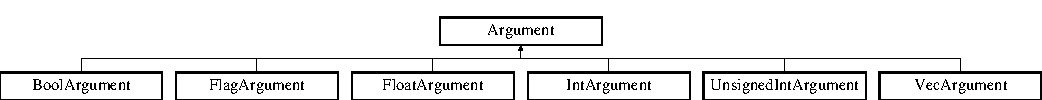
\includegraphics[height=1.342926cm]{classArgument}
\end{center}
\end{figure}
\subsection*{Public Member Functions}
\begin{DoxyCompactItemize}
\item 
\hyperlink{classArgument_ae453df798ec87ee16e61c4cbc2283927}{Argument} (std\-::string l\-Name, char s\-Name, std\-::string descr)
\begin{DoxyCompactList}\small\item\em Constructeur. \end{DoxyCompactList}\item 
char \hyperlink{classArgument_a26b8be0058af34a8c4fc6d5b86cc115f}{get\-Short\-Name} ()
\begin{DoxyCompactList}\small\item\em Accesseur. \end{DoxyCompactList}\item 
std\-::string \hyperlink{classArgument_a9143acb0495de0ec95dede6706aca215}{get\-Long\-Name} ()
\begin{DoxyCompactList}\small\item\em Accesseur. \end{DoxyCompactList}\item 
std\-::string \hyperlink{classArgument_a73e6b45ca7a1049590bbb5b886c72ba5}{get\-Description} ()
\begin{DoxyCompactList}\small\item\em Accesseur. \end{DoxyCompactList}\item 
bool \hyperlink{classArgument_a5dfd49a75fd171250a4997f1605bd638}{get\-Was\-Found} ()
\begin{DoxyCompactList}\small\item\em Accesseur. \end{DoxyCompactList}\item 
void \hyperlink{classArgument_a434158cb4358b10695061128b6e658e7}{set\-Was\-Found} (bool val)
\begin{DoxyCompactList}\small\item\em Mutateur. \end{DoxyCompactList}\item 
std\-::string \hyperlink{classArgument_ac211710802002ea19b3c685028e33177}{get\-Name} (std\-::string type)
\begin{DoxyCompactList}\small\item\em Afficheur. \end{DoxyCompactList}\item 
virtual bool \hyperlink{classArgument_a20b6a0182f1402dd36b20b1a6743e665}{test\-Value} (std\-::string val)=0
\begin{DoxyCompactList}\small\item\em Mutateur et testeur pour m\-\_\-value. \end{DoxyCompactList}\item 
virtual void \hyperlink{classArgument_adab35148c697a617b0b0fcb3169611e3}{display} ()=0
\begin{DoxyCompactList}\small\item\em Afficheur. \end{DoxyCompactList}\item 
virtual \hyperlink{classArgument_a43febc2f1e885cb422849b9bf9012acf}{$\sim$\-Argument} ()
\begin{DoxyCompactList}\small\item\em Destructeur. \end{DoxyCompactList}\end{DoxyCompactItemize}


\subsection{Detailed Description}
Les objets de la classe \hyperlink{classArgument}{Argument} stocke les informations d'un arguments d'une ligne de commande dans plusieurs variables qui sont le nom long de l'argument (m\-\_\-long\-Name), le nom court de l'argument (m\-\_\-short\-Name), la description de l'argument (m\-\_\-description) et une variable booléenne (m\-\_\-was\-Found) qui indique la présence de l'argument dans la ligne de commande. Elle dispose d'un constructeur et de méthodes virtuelles pures qui seront redéfinies dans les sous-\/classes qui permettent de donner la valeur d'un argument (set\-Value()), et d'afficher les informations liées à un argument (\hyperlink{classArgument_adab35148c697a617b0b0fcb3169611e3}{display()}). 

\subsection{Constructor \& Destructor Documentation}
\hypertarget{classArgument_ae453df798ec87ee16e61c4cbc2283927}{\index{Argument@{Argument}!Argument@{Argument}}
\index{Argument@{Argument}!Argument@{Argument}}
\subsubsection[{Argument}]{\setlength{\rightskip}{0pt plus 5cm}Argument\-::\-Argument (
\begin{DoxyParamCaption}
\item[{std\-::string}]{l\-Name, }
\item[{char}]{s\-Name, }
\item[{std\-::string}]{descr}
\end{DoxyParamCaption}
)}}\label{classArgument_ae453df798ec87ee16e61c4cbc2283927}


Constructeur. 


\begin{DoxyParams}{Parameters}
{\em l\-Name} & \-: Nom long de l'argument. \\
\hline
{\em s\-Name} & \-: Nom court de l'argument. \\
\hline
{\em descr} & \-: Description de l'argument.\\
\hline
\end{DoxyParams}
Constructeur de la classe \hyperlink{classArgument}{Argument}. \hypertarget{classArgument_a43febc2f1e885cb422849b9bf9012acf}{\index{Argument@{Argument}!$\sim$\-Argument@{$\sim$\-Argument}}
\index{$\sim$\-Argument@{$\sim$\-Argument}!Argument@{Argument}}
\subsubsection[{$\sim$\-Argument}]{\setlength{\rightskip}{0pt plus 5cm}Argument\-::$\sim$\-Argument (
\begin{DoxyParamCaption}
{}
\end{DoxyParamCaption}
)\hspace{0.3cm}{\ttfamily [inline]}, {\ttfamily [virtual]}}}\label{classArgument_a43febc2f1e885cb422849b9bf9012acf}


Destructeur. 

Destructeur de la classe \hyperlink{classArgument}{Argument} 

\subsection{Member Function Documentation}
\hypertarget{classArgument_adab35148c697a617b0b0fcb3169611e3}{\index{Argument@{Argument}!display@{display}}
\index{display@{display}!Argument@{Argument}}
\subsubsection[{display}]{\setlength{\rightskip}{0pt plus 5cm}void Argument\-::display (
\begin{DoxyParamCaption}
{}
\end{DoxyParamCaption}
)\hspace{0.3cm}{\ttfamily [pure virtual]}}}\label{classArgument_adab35148c697a617b0b0fcb3169611e3}


Afficheur. 

display est une méthode virtuelle pure redéfinie dans les sous-\/classes de la classe \hyperlink{classArgument}{Argument}. C'est une méthode d'affichage d'un argument, l'affichage est sous la forme \-: $<$type$>$ $<$nom$>$ = $<$valeur$>$ 

Implemented in \hyperlink{classVecArgument_ae3611e8947ccbd26681044f20df4b351}{Vec\-Argument}, \hyperlink{classBoolArgument_a458a678ce4c52055f2c09132b49a0aca}{Bool\-Argument}, \hyperlink{classFlagArgument_ab79ece26d0d7462dd491ba0c67bb95d2}{Flag\-Argument}, \hyperlink{classFloatArgument_a25a6f413c78728ffb92b146dce699669}{Float\-Argument}, \hyperlink{classIntArgument_a8bb885657c1f58c1fbacfc513571ea30}{Int\-Argument}, and \hyperlink{classUnsignedIntArgument_a4abf29719479c55ee030821e02699834}{Unsigned\-Int\-Argument}.

\hypertarget{classArgument_a73e6b45ca7a1049590bbb5b886c72ba5}{\index{Argument@{Argument}!get\-Description@{get\-Description}}
\index{get\-Description@{get\-Description}!Argument@{Argument}}
\subsubsection[{get\-Description}]{\setlength{\rightskip}{0pt plus 5cm}string Argument\-::get\-Description (
\begin{DoxyParamCaption}
{}
\end{DoxyParamCaption}
)\hspace{0.3cm}{\ttfamily [inline]}}}\label{classArgument_a73e6b45ca7a1049590bbb5b886c72ba5}


Accesseur. 

\begin{DoxyReturn}{Returns}
La description de l'argument
\end{DoxyReturn}
Accesseur de m\-\_\-description. \hypertarget{classArgument_a9143acb0495de0ec95dede6706aca215}{\index{Argument@{Argument}!get\-Long\-Name@{get\-Long\-Name}}
\index{get\-Long\-Name@{get\-Long\-Name}!Argument@{Argument}}
\subsubsection[{get\-Long\-Name}]{\setlength{\rightskip}{0pt plus 5cm}string Argument\-::get\-Long\-Name (
\begin{DoxyParamCaption}
{}
\end{DoxyParamCaption}
)\hspace{0.3cm}{\ttfamily [inline]}}}\label{classArgument_a9143acb0495de0ec95dede6706aca215}


Accesseur. 

\begin{DoxyReturn}{Returns}
Le nom long de l'argument
\end{DoxyReturn}
Accesseur de m\-\_\-long\-Name. \hypertarget{classArgument_ac211710802002ea19b3c685028e33177}{\index{Argument@{Argument}!get\-Name@{get\-Name}}
\index{get\-Name@{get\-Name}!Argument@{Argument}}
\subsubsection[{get\-Name}]{\setlength{\rightskip}{0pt plus 5cm}std\-::string Argument\-::get\-Name (
\begin{DoxyParamCaption}
\item[{std\-::string}]{type}
\end{DoxyParamCaption}
)}}\label{classArgument_ac211710802002ea19b3c685028e33177}


Afficheur. 


\begin{DoxyParams}{Parameters}
{\em type} & \-: le type à afficher, \char`\"{}\char`\"{} pour aucun type \\
\hline
\end{DoxyParams}
\begin{DoxyReturn}{Returns}
le nom de l'argument sous la forme \-: \char`\"{}-\/nom\-Court \mbox{[}type\mbox{]}, -\/-\/nom\-Long=\mbox{[}type\mbox{]}\char`\"{}
\end{DoxyReturn}
C'est une fonction qui retourne les noms de l'argument sous la forme \-: \char`\"{}nom\-Court, nom\-Long\char`\"{} si type n'est pas précisé. Si un type est précisé cela affiche \char`\"{}-\/nom\-Court type, -\/-\/nom\-Long=type\char`\"{}. \hypertarget{classArgument_a26b8be0058af34a8c4fc6d5b86cc115f}{\index{Argument@{Argument}!get\-Short\-Name@{get\-Short\-Name}}
\index{get\-Short\-Name@{get\-Short\-Name}!Argument@{Argument}}
\subsubsection[{get\-Short\-Name}]{\setlength{\rightskip}{0pt plus 5cm}string Argument\-::get\-Short\-Name (
\begin{DoxyParamCaption}
{}
\end{DoxyParamCaption}
)\hspace{0.3cm}{\ttfamily [inline]}}}\label{classArgument_a26b8be0058af34a8c4fc6d5b86cc115f}


Accesseur. 

\begin{DoxyReturn}{Returns}
Le nom court de l'argument
\end{DoxyReturn}
Accesseur de m\-\_\-short\-Name. \hypertarget{classArgument_a5dfd49a75fd171250a4997f1605bd638}{\index{Argument@{Argument}!get\-Was\-Found@{get\-Was\-Found}}
\index{get\-Was\-Found@{get\-Was\-Found}!Argument@{Argument}}
\subsubsection[{get\-Was\-Found}]{\setlength{\rightskip}{0pt plus 5cm}string Argument\-::get\-Was\-Found (
\begin{DoxyParamCaption}
{}
\end{DoxyParamCaption}
)\hspace{0.3cm}{\ttfamily [inline]}}}\label{classArgument_a5dfd49a75fd171250a4997f1605bd638}


Accesseur. 

\begin{DoxyReturn}{Returns}
Vrai si l'argument est présent dans la ligne de commande, faux sinon
\end{DoxyReturn}
Accesseur de m\-\_\-was\-Found. \hypertarget{classArgument_a434158cb4358b10695061128b6e658e7}{\index{Argument@{Argument}!set\-Was\-Found@{set\-Was\-Found}}
\index{set\-Was\-Found@{set\-Was\-Found}!Argument@{Argument}}
\subsubsection[{set\-Was\-Found}]{\setlength{\rightskip}{0pt plus 5cm}void Argument\-::set\-Was\-Found (
\begin{DoxyParamCaption}
\item[{bool}]{val}
\end{DoxyParamCaption}
)\hspace{0.3cm}{\ttfamily [inline]}}}\label{classArgument_a434158cb4358b10695061128b6e658e7}


Mutateur. 


\begin{DoxyParams}{Parameters}
{\em val} & \-: Booléen indiquant la présence de l'argument ou non dans la ligne de commande\\
\hline
\end{DoxyParams}
Mutateur de m\-\_\-was\-Found. \hypertarget{classArgument_a20b6a0182f1402dd36b20b1a6743e665}{\index{Argument@{Argument}!test\-Value@{test\-Value}}
\index{test\-Value@{test\-Value}!Argument@{Argument}}
\subsubsection[{test\-Value}]{\setlength{\rightskip}{0pt plus 5cm}void Argument\-::test\-Value (
\begin{DoxyParamCaption}
\item[{std\-::string}]{val}
\end{DoxyParamCaption}
)\hspace{0.3cm}{\ttfamily [pure virtual]}}}\label{classArgument_a20b6a0182f1402dd36b20b1a6743e665}


Mutateur et testeur pour m\-\_\-value. 


\begin{DoxyParams}{Parameters}
{\em string} & val \-: valeur à tester \\
\hline
\end{DoxyParams}
\begin{DoxyReturn}{Returns}
Vrai si la valeur est du bon type, faux sinon
\end{DoxyReturn}
test\-Value est une méthode virtuelle pure redéfinie dans les sous-\/classes de la classe \hyperlink{classArgument}{Argument}. C'est une méthode qui prend en paramètre la valeur d'un argument dans la ligne de commande et qui qui place la valeur dans la variable m\-\_\-value et retourne vrai si la valeur est du bon type, faux sinon. 

Implemented in \hyperlink{classVecArgument_a2b3cbbc68d03d2eec8dd00452d228ef1}{Vec\-Argument}, \hyperlink{classBoolArgument_ad4c0bd190cf554294e07d4ad3194308e}{Bool\-Argument}, \hyperlink{classFlagArgument_a881f9de4811858463a4a981d3ebedb79}{Flag\-Argument}, \hyperlink{classFloatArgument_a6456a6760c3030a7c67c688e8cde03be}{Float\-Argument}, \hyperlink{classIntArgument_a3d27054173466542694fd971b13be8bb}{Int\-Argument}, and \hyperlink{classUnsignedIntArgument_a46d930be372e3443fc3f3a2419ceb387}{Unsigned\-Int\-Argument}.



The documentation for this class was generated from the following files\-:\begin{DoxyCompactItemize}
\item 
src/\hyperlink{Argument_8h}{Argument.\-h}\item 
src/\hyperlink{Argument_8cpp}{Argument.\-cpp}\end{DoxyCompactItemize}

\hypertarget{classBoolArgument}{\section{Bool\-Argument Class Reference}
\label{classBoolArgument}\index{Bool\-Argument@{Bool\-Argument}}
}


{\ttfamily \#include $<$Bool\-Argument.\-h$>$}

Inheritance diagram for Bool\-Argument\-:\begin{figure}[H]
\begin{center}
\leavevmode
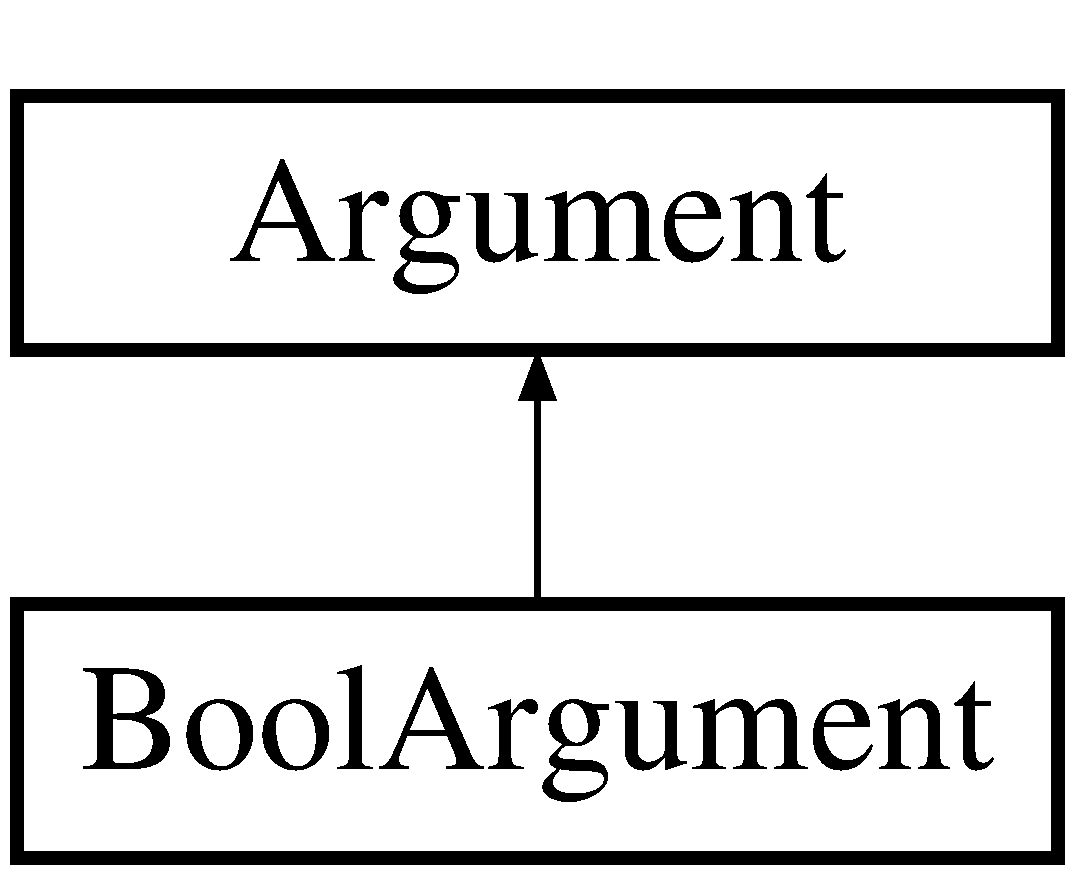
\includegraphics[height=2.000000cm]{classBoolArgument}
\end{center}
\end{figure}
\subsection*{Public Member Functions}
\begin{DoxyCompactItemize}
\item 
\hyperlink{classBoolArgument_aac57d1e4e57f45c6786509ff36f8d274}{Bool\-Argument} (std\-::string l\-Name, char s\-Name, bool $\ast$value, std\-::string descr)
\begin{DoxyCompactList}\small\item\em Constructeur. \end{DoxyCompactList}\item 
bool \hyperlink{classBoolArgument_af51f23cede522a86230b190877d16170}{get\-Value} ()
\begin{DoxyCompactList}\small\item\em Accesseur. \end{DoxyCompactList}\item 
void \hyperlink{classBoolArgument_a7b7c18ef5aee456259062262695dcaa5}{set\-Value} (bool val)
\begin{DoxyCompactList}\small\item\em Mutateur. \end{DoxyCompactList}\item 
bool \hyperlink{classBoolArgument_ad4c0bd190cf554294e07d4ad3194308e}{test\-Value} (std\-::string val)
\begin{DoxyCompactList}\small\item\em Mutateur et testeur. \end{DoxyCompactList}\item 
void \hyperlink{classBoolArgument_a458a678ce4c52055f2c09132b49a0aca}{display} ()
\begin{DoxyCompactList}\small\item\em Afficheur. \end{DoxyCompactList}\item 
\hyperlink{classBoolArgument_a195c1bab8f3e69db0d6170caebced29d}{$\sim$\-Bool\-Argument} ()
\begin{DoxyCompactList}\small\item\em Destructeur. \end{DoxyCompactList}\end{DoxyCompactItemize}


\subsection{Detailed Description}
La classe \hyperlink{classBoolArgument}{Bool\-Argument} hérite de la classe \hyperlink{classArgument}{Argument}. Les objets de cette classe stockent les informations d'un arguments de type booléen, elle posséde une variable qui contient sa valeur (m\-\_\-value). Elle dispose d'un constructeur et des méthodes qui permettent de définir et de tester la valeur d'une instance (\hyperlink{classBoolArgument_ad4c0bd190cf554294e07d4ad3194308e}{test\-Value()}), d'afficher les informations liées à une instance (\hyperlink{classBoolArgument_a458a678ce4c52055f2c09132b49a0aca}{display()}), d'un accesseur (\hyperlink{classBoolArgument_af51f23cede522a86230b190877d16170}{get\-Value()}) et d'un mutateur (\hyperlink{classBoolArgument_a7b7c18ef5aee456259062262695dcaa5}{set\-Value(bool)}). 

\subsection{Constructor \& Destructor Documentation}
\hypertarget{classBoolArgument_aac57d1e4e57f45c6786509ff36f8d274}{\index{Bool\-Argument@{Bool\-Argument}!Bool\-Argument@{Bool\-Argument}}
\index{Bool\-Argument@{Bool\-Argument}!BoolArgument@{Bool\-Argument}}
\subsubsection[{Bool\-Argument}]{\setlength{\rightskip}{0pt plus 5cm}Bool\-Argument\-::\-Bool\-Argument (
\begin{DoxyParamCaption}
\item[{std\-::string}]{l\-Name, }
\item[{char}]{s\-Name, }
\item[{bool $\ast$}]{value, }
\item[{std\-::string}]{descr}
\end{DoxyParamCaption}
)}}\label{classBoolArgument_aac57d1e4e57f45c6786509ff36f8d274}


Constructeur. 


\begin{DoxyParams}{Parameters}
{\em l\-Name} & \-: Nom long de l'argument \\
\hline
{\em s\-Name} & \-: Nom court de l'argument \\
\hline
{\em value} & \-: Pointeur sur le booléen à modifier \\
\hline
{\em descr} & \-: Description de l'argument\\
\hline
\end{DoxyParams}
Constructeur de la classe \hyperlink{classBoolArgument}{Bool\-Argument}. \hypertarget{classBoolArgument_a195c1bab8f3e69db0d6170caebced29d}{\index{Bool\-Argument@{Bool\-Argument}!$\sim$\-Bool\-Argument@{$\sim$\-Bool\-Argument}}
\index{$\sim$\-Bool\-Argument@{$\sim$\-Bool\-Argument}!BoolArgument@{Bool\-Argument}}
\subsubsection[{$\sim$\-Bool\-Argument}]{\setlength{\rightskip}{0pt plus 5cm}Bool\-Argument\-::$\sim$\-Bool\-Argument (
\begin{DoxyParamCaption}
{}
\end{DoxyParamCaption}
)\hspace{0.3cm}{\ttfamily [inline]}}}\label{classBoolArgument_a195c1bab8f3e69db0d6170caebced29d}


Destructeur. 

Destructeur de la classe \hyperlink{classBoolArgument}{Bool\-Argument} 

\subsection{Member Function Documentation}
\hypertarget{classBoolArgument_a458a678ce4c52055f2c09132b49a0aca}{\index{Bool\-Argument@{Bool\-Argument}!display@{display}}
\index{display@{display}!BoolArgument@{Bool\-Argument}}
\subsubsection[{display}]{\setlength{\rightskip}{0pt plus 5cm}void Bool\-Argument\-::display (
\begin{DoxyParamCaption}
{}
\end{DoxyParamCaption}
)\hspace{0.3cm}{\ttfamily [virtual]}}}\label{classBoolArgument_a458a678ce4c52055f2c09132b49a0aca}


Afficheur. 

C'est une méthode d'affichage d'un argument, l'affichage est sous la forme \-: Bool $<$nom$>$ = $<$valeur$>$ 

Implements \hyperlink{classArgument_adab35148c697a617b0b0fcb3169611e3}{Argument}.

\hypertarget{classBoolArgument_af51f23cede522a86230b190877d16170}{\index{Bool\-Argument@{Bool\-Argument}!get\-Value@{get\-Value}}
\index{get\-Value@{get\-Value}!BoolArgument@{Bool\-Argument}}
\subsubsection[{get\-Value}]{\setlength{\rightskip}{0pt plus 5cm}bool Bool\-Argument\-::get\-Value (
\begin{DoxyParamCaption}
{}
\end{DoxyParamCaption}
)\hspace{0.3cm}{\ttfamily [inline]}}}\label{classBoolArgument_af51f23cede522a86230b190877d16170}


Accesseur. 

\begin{DoxyReturn}{Returns}
Valeur de l'argument
\end{DoxyReturn}
Accesseur de m\-\_\-value. \hypertarget{classBoolArgument_a7b7c18ef5aee456259062262695dcaa5}{\index{Bool\-Argument@{Bool\-Argument}!set\-Value@{set\-Value}}
\index{set\-Value@{set\-Value}!BoolArgument@{Bool\-Argument}}
\subsubsection[{set\-Value}]{\setlength{\rightskip}{0pt plus 5cm}void Bool\-Argument\-::set\-Value (
\begin{DoxyParamCaption}
\item[{bool}]{val}
\end{DoxyParamCaption}
)\hspace{0.3cm}{\ttfamily [inline]}}}\label{classBoolArgument_a7b7c18ef5aee456259062262695dcaa5}


Mutateur. 


\begin{DoxyParams}{Parameters}
{\em val} & \-: Booléen qui donnera sa valeur à la variable m\-\_\-value.\\
\hline
\end{DoxyParams}
Mutateur de m\-\_\-value. \hypertarget{classBoolArgument_ad4c0bd190cf554294e07d4ad3194308e}{\index{Bool\-Argument@{Bool\-Argument}!test\-Value@{test\-Value}}
\index{test\-Value@{test\-Value}!BoolArgument@{Bool\-Argument}}
\subsubsection[{test\-Value}]{\setlength{\rightskip}{0pt plus 5cm}bool Bool\-Argument\-::test\-Value (
\begin{DoxyParamCaption}
\item[{std\-::string}]{val}
\end{DoxyParamCaption}
)\hspace{0.3cm}{\ttfamily [virtual]}}}\label{classBoolArgument_ad4c0bd190cf554294e07d4ad3194308e}


Mutateur et testeur. 


\begin{DoxyParams}{Parameters}
{\em val} & \-: valeur d'un argument \\
\hline
\end{DoxyParams}
\begin{DoxyReturn}{Returns}
Vrai si la valeur est du bon type, faux sinon.
\end{DoxyReturn}
C'est une méthode qui prend en paramètre la valeur d'un argument via la ligne de commande et qui test si elle correspond bien à un booléen. Si c'est le cas, la méthode met la valeur dans l'instance et retourne vrai, sinon faux. 

Implements \hyperlink{classArgument_a20b6a0182f1402dd36b20b1a6743e665}{Argument}.



The documentation for this class was generated from the following files\-:\begin{DoxyCompactItemize}
\item 
src/\hyperlink{BoolArgument_8h}{Bool\-Argument.\-h}\item 
src/\hyperlink{BoolArgument_8cpp}{Bool\-Argument.\-cpp}\end{DoxyCompactItemize}

\hypertarget{classCommandLine}{\section{Command\-Line Class Reference}
\label{classCommandLine}\index{Command\-Line@{Command\-Line}}
}


{\ttfamily \#include $<$Command\-Line.\-h$>$}

\subsection*{Public Member Functions}
\begin{DoxyCompactItemize}
\item 
\hyperlink{classCommandLine_ae6329212e2108a9e2a1795f27fab33eb}{Command\-Line} ()
\begin{DoxyCompactList}\small\item\em Constructeur. \end{DoxyCompactList}\item 
\hyperlink{classCommandLine_ab996878223010dc05cac5e21606e0671}{Command\-Line} (unsigned int argc, char $\ast$$\ast$argv)
\begin{DoxyCompactList}\small\item\em Constructeur. \end{DoxyCompactList}\item 
\hypertarget{classCommandLine_a8d677ccd88e53ba3e1c01936a39d231d}{void {\bfseries set\-Arg\-C} (unsigned int val)}\label{classCommandLine_a8d677ccd88e53ba3e1c01936a39d231d}

\item 
\hypertarget{classCommandLine_a3e5dc0a46e7faa50564b3df18f6456bb}{void {\bfseries set\-Arg\-V} (char $\ast$$\ast$val)}\label{classCommandLine_a3e5dc0a46e7faa50564b3df18f6456bb}

\item 
\hypertarget{classCommandLine_a392affafb13a71b1ec6c731e37f65954}{std\-::vector$<$ \hyperlink{classArgument}{Argument} $\ast$ $>$ {\bfseries get\-Vec\-Arg} ()}\label{classCommandLine_a392affafb13a71b1ec6c731e37f65954}

\item 
void \hyperlink{classCommandLine_a3cd1954c5c82980a3f57288d09192937}{add} (\hyperlink{classArgument}{Argument} $\ast$a)
\item 
\hyperlink{classArgument}{Argument} $\ast$ \hyperlink{classCommandLine_a884050a7939bd56a166001f162fbfc7b}{find} (char $\ast$name)
\item 
bool \hyperlink{classCommandLine_a62cd80cf6f4f99867034ce43c2c1b94f}{parse} ()
\item 
\hypertarget{classCommandLine_a611e230a49e8fccc31410aad81c88991}{void \hyperlink{classCommandLine_a611e230a49e8fccc31410aad81c88991}{display} ()}\label{classCommandLine_a611e230a49e8fccc31410aad81c88991}

\begin{DoxyCompactList}\small\item\em Afficheur

C'est une méthode d'affichage, elle parcours le vecteur d'arguments en entier pour afficher chaques éléments de celui-\/ci, s'ils sont présent dans la ligne de commande. \end{DoxyCompactList}\item 
\hypertarget{classCommandLine_a5c75f2e2c604253a476134e0427ede57}{void \hyperlink{classCommandLine_a5c75f2e2c604253a476134e0427ede57}{display\-All} ()}\label{classCommandLine_a5c75f2e2c604253a476134e0427ede57}

\begin{DoxyCompactList}\small\item\em Afficheur

C'est une méthode d'affichage, elle parcours le vecteur d'arguments en entier pour afficher chaques éléments de celui-\/ci. \end{DoxyCompactList}\item 
std\-::string \hyperlink{classCommandLine_a9611a3048e9ce31c91c23a18c6143c60}{get\-Choix\-Arg} (\hyperlink{classArgument}{Argument} $\ast$arg)
\item 
void \hyperlink{classCommandLine_abcbfd8d82d87a58776ce92c1f36f8432}{Return\-At\-Line} (std\-::string s, unsigned int nb\-\_\-tab)
\item 
void \hyperlink{classCommandLine_af1ccfe2c88a4eb39136f94d96592525a}{print\-\_\-synopsis} (std\-::string commande, std\-::string description)
\item 
\hyperlink{classCommandLine_ac359efccafe57f845b1f747a9db3c6d9}{$\sim$\-Command\-Line} ()
\begin{DoxyCompactList}\small\item\em Destructeur. \end{DoxyCompactList}\end{DoxyCompactItemize}


\subsection{Detailed Description}
Les objets de la classe \hyperlink{classCommandLine}{Command\-Line} stocke les informations d'une ligne de commande comme le nombre d'arguments dans la ligne (m\-\_\-argc) et les arguments eux-\/même dans un tableau (m\-\_\-argv), ainsi qu'un vecteur d'argument (m\-\_\-vec\-Arg). La classe possède un constructeur, un destructeur et des méthodes de gestions d'arguments qui permettent \-: d'ajouter un argument dans le vecteur d'argument (add(\-Argument)), de trouver si un argument est court ou long et si il est présent dans le vecteur (\hyperlink{classCommandLine_a884050a7939bd56a166001f162fbfc7b}{find(char$\ast$)}), de tester si un argument est une option courte ou longue et si elle est suivie d'une valeur (\hyperlink{classCommandLine_a62cd80cf6f4f99867034ce43c2c1b94f}{parse()}), et une méthode d'affichage des éléments du vecteurs (\hyperlink{classCommandLine_a611e230a49e8fccc31410aad81c88991}{display()}). 

\subsection{Constructor \& Destructor Documentation}
\hypertarget{classCommandLine_ae6329212e2108a9e2a1795f27fab33eb}{\index{Command\-Line@{Command\-Line}!Command\-Line@{Command\-Line}}
\index{Command\-Line@{Command\-Line}!CommandLine@{Command\-Line}}
\subsubsection[{Command\-Line}]{\setlength{\rightskip}{0pt plus 5cm}Command\-Line\-::\-Command\-Line (
\begin{DoxyParamCaption}
{}
\end{DoxyParamCaption}
)}}\label{classCommandLine_ae6329212e2108a9e2a1795f27fab33eb}


Constructeur. 

Constructeur de la classe \hyperlink{classCommandLine}{Command\-Line} \hypertarget{classCommandLine_ab996878223010dc05cac5e21606e0671}{\index{Command\-Line@{Command\-Line}!Command\-Line@{Command\-Line}}
\index{Command\-Line@{Command\-Line}!CommandLine@{Command\-Line}}
\subsubsection[{Command\-Line}]{\setlength{\rightskip}{0pt plus 5cm}Command\-Line\-::\-Command\-Line (
\begin{DoxyParamCaption}
\item[{unsigned int}]{argc, }
\item[{char $\ast$$\ast$}]{argv}
\end{DoxyParamCaption}
)}}\label{classCommandLine_ab996878223010dc05cac5e21606e0671}


Constructeur. 


\begin{DoxyParams}{Parameters}
{\em argc} & \-: nombre d'argument de la ligne de commande \\
\hline
{\em argv} & \-: tableau des arguments de la ligne de commande\\
\hline
\end{DoxyParams}
Constructeur de la classe \hyperlink{classCommandLine}{Command\-Line} \hypertarget{classCommandLine_ac359efccafe57f845b1f747a9db3c6d9}{\index{Command\-Line@{Command\-Line}!$\sim$\-Command\-Line@{$\sim$\-Command\-Line}}
\index{$\sim$\-Command\-Line@{$\sim$\-Command\-Line}!CommandLine@{Command\-Line}}
\subsubsection[{$\sim$\-Command\-Line}]{\setlength{\rightskip}{0pt plus 5cm}Command\-Line\-::$\sim$\-Command\-Line (
\begin{DoxyParamCaption}
{}
\end{DoxyParamCaption}
)}}\label{classCommandLine_ac359efccafe57f845b1f747a9db3c6d9}


Destructeur. 

Destructeur de la classe \hyperlink{classCommandLine}{Command\-Line}. 

\subsection{Member Function Documentation}
\hypertarget{classCommandLine_a3cd1954c5c82980a3f57288d09192937}{\index{Command\-Line@{Command\-Line}!add@{add}}
\index{add@{add}!CommandLine@{Command\-Line}}
\subsubsection[{add}]{\setlength{\rightskip}{0pt plus 5cm}void Command\-Line\-::add (
\begin{DoxyParamCaption}
\item[{{\bf Argument} $\ast$}]{a}
\end{DoxyParamCaption}
)}}\label{classCommandLine_a3cd1954c5c82980a3f57288d09192937}

\begin{DoxyParams}{Parameters}
{\em $\ast$a} & \-: pointeur sur un argument.\\
\hline
\end{DoxyParams}
C'est une méthode qui permet d'ajouter un argument au vecteur d'arguments (m\-\_\-vec\-Arg). \hypertarget{classCommandLine_a884050a7939bd56a166001f162fbfc7b}{\index{Command\-Line@{Command\-Line}!find@{find}}
\index{find@{find}!CommandLine@{Command\-Line}}
\subsubsection[{find}]{\setlength{\rightskip}{0pt plus 5cm}{\bf Argument} $\ast$ Command\-Line\-::find (
\begin{DoxyParamCaption}
\item[{char $\ast$}]{name}
\end{DoxyParamCaption}
)}}\label{classCommandLine_a884050a7939bd56a166001f162fbfc7b}

\begin{DoxyParams}{Parameters}
{\em name} & \-: nom d'un argument en chaine de caractère \\
\hline
\end{DoxyParams}
\begin{DoxyReturn}{Returns}
Pointeur sur argument si la méthode à trouvé cet argument, N\-U\-L\-L sinon.
\end{DoxyReturn}
C'est une méthode qui prend le nom d'un argument en paramètre et qui recherche sa présence dans le vecteur d'arguments (m\-\_\-vec\-Arg) et qui retourne un pointeur sur cet argument si la méthode l'a trouvé, sinon elle retourne la valeur N\-U\-L\-L. \hypertarget{classCommandLine_a9611a3048e9ce31c91c23a18c6143c60}{\index{Command\-Line@{Command\-Line}!get\-Choix\-Arg@{get\-Choix\-Arg}}
\index{get\-Choix\-Arg@{get\-Choix\-Arg}!CommandLine@{Command\-Line}}
\subsubsection[{get\-Choix\-Arg}]{\setlength{\rightskip}{0pt plus 5cm}string Command\-Line\-::get\-Choix\-Arg (
\begin{DoxyParamCaption}
\item[{{\bf Argument} $\ast$}]{arg}
\end{DoxyParamCaption}
)}}\label{classCommandLine_a9611a3048e9ce31c91c23a18c6143c60}

\begin{DoxyParams}{Parameters}
{\em arg} & \-: l'argument sur lequel on test \\
\hline
\end{DoxyParams}
\begin{DoxyReturn}{Returns}
Les choix correspondant à la référence d'un argument en chaîne de caractère.
\end{DoxyReturn}
C'est une méthode qui prend une référence à un argument en paramètre et qui test si le type de la classe correspond à un type existant tel que bool, int, float, unsigned int ou vector, et qui retourne les types possibles en chaîne de caractère. \hypertarget{classCommandLine_a62cd80cf6f4f99867034ce43c2c1b94f}{\index{Command\-Line@{Command\-Line}!parse@{parse}}
\index{parse@{parse}!CommandLine@{Command\-Line}}
\subsubsection[{parse}]{\setlength{\rightskip}{0pt plus 5cm}bool Command\-Line\-::parse (
\begin{DoxyParamCaption}
{}
\end{DoxyParamCaption}
)}}\label{classCommandLine_a62cd80cf6f4f99867034ce43c2c1b94f}
\begin{DoxyReturn}{Returns}
Vrai si l'argument est suivie d'une valeur du bon type, faux sinon.
\end{DoxyReturn}
C'est une méthode qui teste si un argument est une option courte ou longue et si la valeur suivant l'argument est d'un type correcte. Donc elle retourne vrai si tout c'est bien passé, ou faux si une erreur survient lors d'une opération. \hypertarget{classCommandLine_af1ccfe2c88a4eb39136f94d96592525a}{\index{Command\-Line@{Command\-Line}!print\-\_\-synopsis@{print\-\_\-synopsis}}
\index{print\-\_\-synopsis@{print\-\_\-synopsis}!CommandLine@{Command\-Line}}
\subsubsection[{print\-\_\-synopsis}]{\setlength{\rightskip}{0pt plus 5cm}void Command\-Line\-::print\-\_\-synopsis (
\begin{DoxyParamCaption}
\item[{std\-::string}]{commande, }
\item[{std\-::string}]{description}
\end{DoxyParamCaption}
)}}\label{classCommandLine_af1ccfe2c88a4eb39136f94d96592525a}
C'est une méthode qui prend en paramètre le nom du programme et sa description et qui affiche toute les possibilités d'éxécution possibles, ainsi qu'une description pour chaques arguments possibles. \hypertarget{classCommandLine_abcbfd8d82d87a58776ce92c1f36f8432}{\index{Command\-Line@{Command\-Line}!Return\-At\-Line@{Return\-At\-Line}}
\index{Return\-At\-Line@{Return\-At\-Line}!CommandLine@{Command\-Line}}
\subsubsection[{Return\-At\-Line}]{\setlength{\rightskip}{0pt plus 5cm}void Command\-Line\-::\-Return\-At\-Line (
\begin{DoxyParamCaption}
\item[{std\-::string}]{s, }
\item[{unsigned int}]{nb\-\_\-tab}
\end{DoxyParamCaption}
)}}\label{classCommandLine_abcbfd8d82d87a58776ce92c1f36f8432}

\begin{DoxyParams}{Parameters}
{\em ch} & \-: La chaine de caractère contenant le nom du programme et sa description, nb\-\_\-tab \-: le nombre de tabulation.\\
\hline
\end{DoxyParams}
C'est une méthode qui prend une chaîne de caractère contenant le nom du programme et sa description en paramètre et qui permet de les mettre en page, c'est à dire qu'il insère les tabulations en début de ligne et qu'il retourne à la ligne quand la chaîne de caractère $\ast$ dépasse les 60 caractères par ligne (avec découpage au mot). 

The documentation for this class was generated from the following files\-:\begin{DoxyCompactItemize}
\item 
src/\hyperlink{CommandLine_8h}{Command\-Line.\-h}\item 
src/\hyperlink{CommandLine_8cpp}{Command\-Line.\-cpp}\end{DoxyCompactItemize}

\hypertarget{classFlagArgument}{\section{Flag\-Argument Class Reference}
\label{classFlagArgument}\index{Flag\-Argument@{Flag\-Argument}}
}


{\ttfamily \#include $<$Flag\-Argument.\-h$>$}

Inheritance diagram for Flag\-Argument\-:\begin{figure}[H]
\begin{center}
\leavevmode
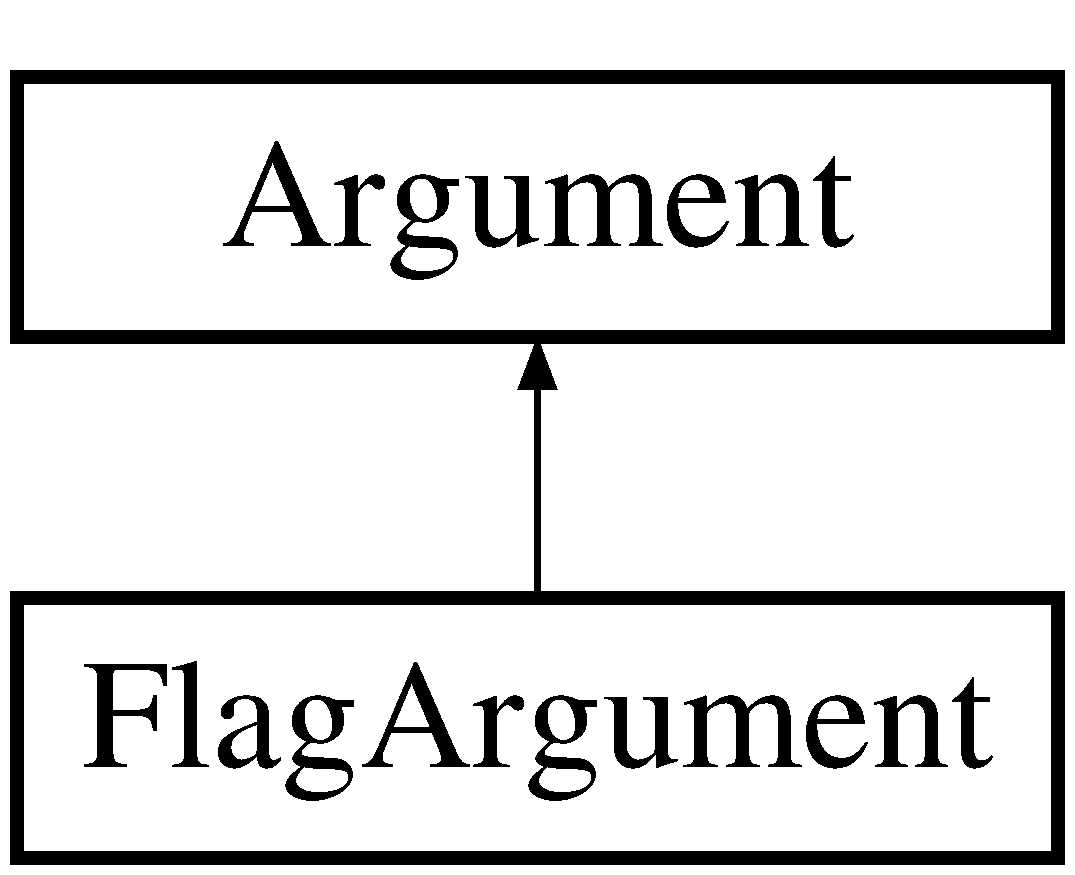
\includegraphics[height=2.000000cm]{classFlagArgument}
\end{center}
\end{figure}
\subsection*{Public Member Functions}
\begin{DoxyCompactItemize}
\item 
\hyperlink{classFlagArgument_aef16024973942f8be515c430e0a90c66}{Flag\-Argument} (std\-::string l\-Name, char s\-Name, bool $\ast$value, std\-::string descr)
\begin{DoxyCompactList}\small\item\em Constructeur. \end{DoxyCompactList}\item 
bool \hyperlink{classFlagArgument_a78f4e074860e7a358097e0b3814aab3f}{get\-Value} ()
\begin{DoxyCompactList}\small\item\em Accesseur. \end{DoxyCompactList}\item 
void \hyperlink{classFlagArgument_ab663d3b44ceb27bb2cee27b91f13363d}{set\-Value} (bool val)
\begin{DoxyCompactList}\small\item\em Mutateur. \end{DoxyCompactList}\item 
bool \hyperlink{classFlagArgument_a881f9de4811858463a4a981d3ebedb79}{test\-Value} (std\-::string val)
\begin{DoxyCompactList}\small\item\em Mutateur et testeur. \end{DoxyCompactList}\item 
void \hyperlink{classFlagArgument_ab79ece26d0d7462dd491ba0c67bb95d2}{display} ()
\begin{DoxyCompactList}\small\item\em Afficheur. \end{DoxyCompactList}\end{DoxyCompactItemize}


\subsection{Detailed Description}
La classe \hyperlink{classFlagArgument}{Flag\-Argument} hérite de la classe \hyperlink{classArgument}{Argument}. Les objets de cette classe stockent les informations d'un arguments de type booléen, elle posséde une variable qui contient sa valeur (m\-\_\-value). Elle dispose d'un constructeur et des méthodes qui permettent de définir et de tester la valeur d'une instance (\hyperlink{classFlagArgument_a881f9de4811858463a4a981d3ebedb79}{test\-Value()}), d'afficher les informations liées à une instance (\hyperlink{classFlagArgument_ab79ece26d0d7462dd491ba0c67bb95d2}{display()}), d'un accesseur (\hyperlink{classFlagArgument_a78f4e074860e7a358097e0b3814aab3f}{get\-Value()}) et d'un mutateur (\hyperlink{classFlagArgument_ab663d3b44ceb27bb2cee27b91f13363d}{set\-Value(bool)}). 

\subsection{Constructor \& Destructor Documentation}
\hypertarget{classFlagArgument_aef16024973942f8be515c430e0a90c66}{\index{Flag\-Argument@{Flag\-Argument}!Flag\-Argument@{Flag\-Argument}}
\index{Flag\-Argument@{Flag\-Argument}!FlagArgument@{Flag\-Argument}}
\subsubsection[{Flag\-Argument}]{\setlength{\rightskip}{0pt plus 5cm}Flag\-Argument\-::\-Flag\-Argument (
\begin{DoxyParamCaption}
\item[{std\-::string}]{l\-Name, }
\item[{char}]{s\-Name, }
\item[{bool $\ast$}]{value, }
\item[{std\-::string}]{descr}
\end{DoxyParamCaption}
)}}\label{classFlagArgument_aef16024973942f8be515c430e0a90c66}


Constructeur. 


\begin{DoxyParams}{Parameters}
{\em l\-Name} & \-: Nom long de l'argument \\
\hline
{\em s\-Name} & \-: Nom court de l'argument \\
\hline
{\em value} & \-: Pointeur sur le booléen à modifier \\
\hline
{\em descr} & \-: Description de l'argument\\
\hline
\end{DoxyParams}
Constructeur de la classe \hyperlink{classBoolArgument}{Bool\-Argument}. 

\subsection{Member Function Documentation}
\hypertarget{classFlagArgument_ab79ece26d0d7462dd491ba0c67bb95d2}{\index{Flag\-Argument@{Flag\-Argument}!display@{display}}
\index{display@{display}!FlagArgument@{Flag\-Argument}}
\subsubsection[{display}]{\setlength{\rightskip}{0pt plus 5cm}void Flag\-Argument\-::display (
\begin{DoxyParamCaption}
{}
\end{DoxyParamCaption}
)\hspace{0.3cm}{\ttfamily [virtual]}}}\label{classFlagArgument_ab79ece26d0d7462dd491ba0c67bb95d2}


Afficheur. 

C'est une méthode d'affichage d'un argument, l'affichage est sous la forme \-: Bool $<$nom$>$ = $<$valeur$>$ 

Implements \hyperlink{classArgument_adab35148c697a617b0b0fcb3169611e3}{Argument}.

\hypertarget{classFlagArgument_a78f4e074860e7a358097e0b3814aab3f}{\index{Flag\-Argument@{Flag\-Argument}!get\-Value@{get\-Value}}
\index{get\-Value@{get\-Value}!FlagArgument@{Flag\-Argument}}
\subsubsection[{get\-Value}]{\setlength{\rightskip}{0pt plus 5cm}bool Flag\-Argument\-::get\-Value (
\begin{DoxyParamCaption}
{}
\end{DoxyParamCaption}
)\hspace{0.3cm}{\ttfamily [inline]}}}\label{classFlagArgument_a78f4e074860e7a358097e0b3814aab3f}


Accesseur. 

\begin{DoxyReturn}{Returns}
Valeur de l'argument
\end{DoxyReturn}
Accesseur de m\-\_\-value. \hypertarget{classFlagArgument_ab663d3b44ceb27bb2cee27b91f13363d}{\index{Flag\-Argument@{Flag\-Argument}!set\-Value@{set\-Value}}
\index{set\-Value@{set\-Value}!FlagArgument@{Flag\-Argument}}
\subsubsection[{set\-Value}]{\setlength{\rightskip}{0pt plus 5cm}void Flag\-Argument\-::set\-Value (
\begin{DoxyParamCaption}
\item[{bool}]{val}
\end{DoxyParamCaption}
)\hspace{0.3cm}{\ttfamily [inline]}}}\label{classFlagArgument_ab663d3b44ceb27bb2cee27b91f13363d}


Mutateur. 


\begin{DoxyParams}{Parameters}
{\em val} & \-: Booléen qui donnera sa valeur à la variable m\-\_\-value.\\
\hline
\end{DoxyParams}
Mutateur de m\-\_\-value. \hypertarget{classFlagArgument_a881f9de4811858463a4a981d3ebedb79}{\index{Flag\-Argument@{Flag\-Argument}!test\-Value@{test\-Value}}
\index{test\-Value@{test\-Value}!FlagArgument@{Flag\-Argument}}
\subsubsection[{test\-Value}]{\setlength{\rightskip}{0pt plus 5cm}bool Flag\-Argument\-::test\-Value (
\begin{DoxyParamCaption}
\item[{std\-::string}]{val}
\end{DoxyParamCaption}
)\hspace{0.3cm}{\ttfamily [virtual]}}}\label{classFlagArgument_a881f9de4811858463a4a981d3ebedb79}


Mutateur et testeur. 


\begin{DoxyParams}{Parameters}
{\em val} & \-: valeur d'un argument \\
\hline
\end{DoxyParams}
\begin{DoxyReturn}{Returns}
Vrai si la valeur est du bon type, faux sinon.
\end{DoxyReturn}
C'est une méthode qui prend en paramètre la valeur d'un argument via la ligne de commande et qui test si elle correspond bien à un booléen. Si c'est le cas, la méthode met la valeur dans l'instance et retourne vrai, sinon faux. 

Implements \hyperlink{classArgument_a20b6a0182f1402dd36b20b1a6743e665}{Argument}.



The documentation for this class was generated from the following files\-:\begin{DoxyCompactItemize}
\item 
src/\hyperlink{FlagArgument_8h}{Flag\-Argument.\-h}\item 
src/\hyperlink{FlagArgument_8cpp}{Flag\-Argument.\-cpp}\end{DoxyCompactItemize}

\hypertarget{classFloatArgument}{\section{Float\-Argument Class Reference}
\label{classFloatArgument}\index{Float\-Argument@{Float\-Argument}}
}


{\ttfamily \#include $<$Float\-Argument.\-h$>$}

Inheritance diagram for Float\-Argument\-:\begin{figure}[H]
\begin{center}
\leavevmode
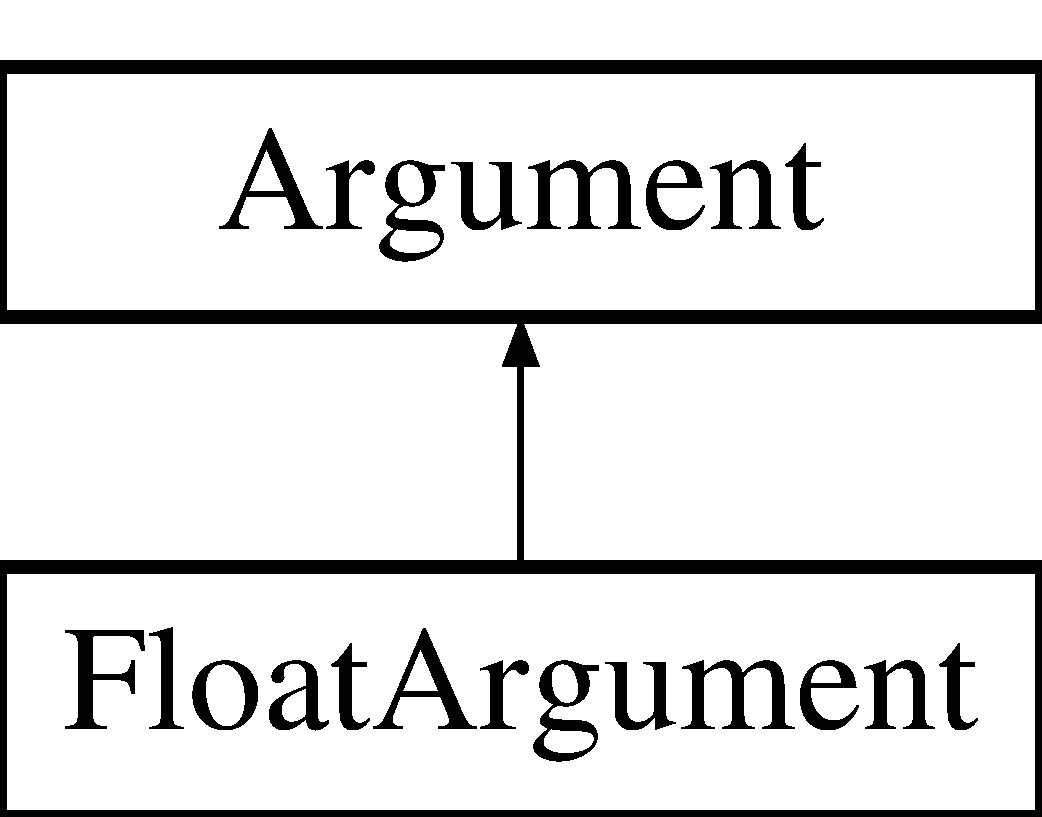
\includegraphics[height=2.000000cm]{classFloatArgument}
\end{center}
\end{figure}
\subsection*{Public Member Functions}
\begin{DoxyCompactItemize}
\item 
\hyperlink{classFloatArgument_a8d62a9520880a965646eccb244c0befb}{Float\-Argument} (std\-::string l\-Name, char s\-Name, float $\ast$value, std\-::string descr)
\begin{DoxyCompactList}\small\item\em Constructeur. \end{DoxyCompactList}\item 
float \hyperlink{classFloatArgument_a304c4a066b705321c11c522cdbf27818}{get\-Value} ()
\begin{DoxyCompactList}\small\item\em Accesseur. \end{DoxyCompactList}\item 
void \hyperlink{classFloatArgument_a3a975e03f230f16346507b90fa598ef0}{set\-Value} (float val)
\begin{DoxyCompactList}\small\item\em Mutateur. \end{DoxyCompactList}\item 
bool \hyperlink{classFloatArgument_a6456a6760c3030a7c67c688e8cde03be}{test\-Value} (std\-::string val)
\begin{DoxyCompactList}\small\item\em Mutateur et testeur. \end{DoxyCompactList}\item 
void \hyperlink{classFloatArgument_a25a6f413c78728ffb92b146dce699669}{display} ()
\begin{DoxyCompactList}\small\item\em Afficheur. \end{DoxyCompactList}\item 
\hyperlink{classFloatArgument_a6c5c8db366c42123d2b021a1cc540717}{$\sim$\-Float\-Argument} ()
\begin{DoxyCompactList}\small\item\em Destructeur. \end{DoxyCompactList}\end{DoxyCompactItemize}


\subsection{Detailed Description}
La classe \hyperlink{classFloatArgument}{Float\-Argument} hérite de la classe \hyperlink{classArgument}{Argument}. Les objets de cette classe stockent les informations d'un argument de type float, elle posséde une variable qui contient sa valeur (m\-\_\-value). Elle dispose d'un constructeur et des méthodes qui permettent de tester et de définir la valeur d'une instance (\hyperlink{classFloatArgument_a6456a6760c3030a7c67c688e8cde03be}{test\-Value()}), d'afficher les informations liées à une instance (\hyperlink{classFloatArgument_a25a6f413c78728ffb92b146dce699669}{display()}), d'un accesseur (\hyperlink{classFloatArgument_a304c4a066b705321c11c522cdbf27818}{get\-Value()}) et d'un mutateur (\hyperlink{classFloatArgument_a3a975e03f230f16346507b90fa598ef0}{set\-Value(float)}). 

\subsection{Constructor \& Destructor Documentation}
\hypertarget{classFloatArgument_a8d62a9520880a965646eccb244c0befb}{\index{Float\-Argument@{Float\-Argument}!Float\-Argument@{Float\-Argument}}
\index{Float\-Argument@{Float\-Argument}!FloatArgument@{Float\-Argument}}
\subsubsection[{Float\-Argument}]{\setlength{\rightskip}{0pt plus 5cm}Float\-Argument\-::\-Float\-Argument (
\begin{DoxyParamCaption}
\item[{std\-::string}]{l\-Name, }
\item[{char}]{s\-Name, }
\item[{float $\ast$}]{value, }
\item[{std\-::string}]{descr}
\end{DoxyParamCaption}
)}}\label{classFloatArgument_a8d62a9520880a965646eccb244c0befb}


Constructeur. 


\begin{DoxyParams}{Parameters}
{\em l\-Name} & \-: Nom long de l'argument \\
\hline
{\em s\-Name} & \-: Nom court de l'argument \\
\hline
{\em value} & \-: Pointeur sur le float à modifier \\
\hline
{\em descr} & \-: Description de l'argument\\
\hline
\end{DoxyParams}
Constructeur de la classe \hyperlink{classFloatArgument}{Float\-Argument}. \hypertarget{classFloatArgument_a6c5c8db366c42123d2b021a1cc540717}{\index{Float\-Argument@{Float\-Argument}!$\sim$\-Float\-Argument@{$\sim$\-Float\-Argument}}
\index{$\sim$\-Float\-Argument@{$\sim$\-Float\-Argument}!FloatArgument@{Float\-Argument}}
\subsubsection[{$\sim$\-Float\-Argument}]{\setlength{\rightskip}{0pt plus 5cm}Float\-Argument\-::$\sim$\-Float\-Argument (
\begin{DoxyParamCaption}
{}
\end{DoxyParamCaption}
)\hspace{0.3cm}{\ttfamily [inline]}}}\label{classFloatArgument_a6c5c8db366c42123d2b021a1cc540717}


Destructeur. 

Destructeur de la classe \hyperlink{classFloatArgument}{Float\-Argument} 

\subsection{Member Function Documentation}
\hypertarget{classFloatArgument_a25a6f413c78728ffb92b146dce699669}{\index{Float\-Argument@{Float\-Argument}!display@{display}}
\index{display@{display}!FloatArgument@{Float\-Argument}}
\subsubsection[{display}]{\setlength{\rightskip}{0pt plus 5cm}void Float\-Argument\-::display (
\begin{DoxyParamCaption}
{}
\end{DoxyParamCaption}
)\hspace{0.3cm}{\ttfamily [virtual]}}}\label{classFloatArgument_a25a6f413c78728ffb92b146dce699669}


Afficheur. 

C'est une méthode d'affichage d'un argument, l'affichage est sous la forme \-: Float $<$nom$>$ = $<$valeur$>$ 

Implements \hyperlink{classArgument_adab35148c697a617b0b0fcb3169611e3}{Argument}.

\hypertarget{classFloatArgument_a304c4a066b705321c11c522cdbf27818}{\index{Float\-Argument@{Float\-Argument}!get\-Value@{get\-Value}}
\index{get\-Value@{get\-Value}!FloatArgument@{Float\-Argument}}
\subsubsection[{get\-Value}]{\setlength{\rightskip}{0pt plus 5cm}bool Float\-Argument\-::get\-Value (
\begin{DoxyParamCaption}
{}
\end{DoxyParamCaption}
)\hspace{0.3cm}{\ttfamily [inline]}}}\label{classFloatArgument_a304c4a066b705321c11c522cdbf27818}


Accesseur. 

\begin{DoxyReturn}{Returns}
Valeur de l'argument
\end{DoxyReturn}
Accesseur de m\-\_\-value. \hypertarget{classFloatArgument_a3a975e03f230f16346507b90fa598ef0}{\index{Float\-Argument@{Float\-Argument}!set\-Value@{set\-Value}}
\index{set\-Value@{set\-Value}!FloatArgument@{Float\-Argument}}
\subsubsection[{set\-Value}]{\setlength{\rightskip}{0pt plus 5cm}void Float\-Argument\-::set\-Value (
\begin{DoxyParamCaption}
\item[{float}]{val}
\end{DoxyParamCaption}
)\hspace{0.3cm}{\ttfamily [inline]}}}\label{classFloatArgument_a3a975e03f230f16346507b90fa598ef0}


Mutateur. 


\begin{DoxyParams}{Parameters}
{\em val} & \-: Float qui donnera sa valeur à la variable m\-\_\-value.\\
\hline
\end{DoxyParams}
Mutateur de m\-\_\-value. \hypertarget{classFloatArgument_a6456a6760c3030a7c67c688e8cde03be}{\index{Float\-Argument@{Float\-Argument}!test\-Value@{test\-Value}}
\index{test\-Value@{test\-Value}!FloatArgument@{Float\-Argument}}
\subsubsection[{test\-Value}]{\setlength{\rightskip}{0pt plus 5cm}bool Float\-Argument\-::test\-Value (
\begin{DoxyParamCaption}
\item[{std\-::string}]{val}
\end{DoxyParamCaption}
)\hspace{0.3cm}{\ttfamily [virtual]}}}\label{classFloatArgument_a6456a6760c3030a7c67c688e8cde03be}


Mutateur et testeur. 


\begin{DoxyParams}{Parameters}
{\em val} & \-: valeur d'un argument \\
\hline
\end{DoxyParams}
\begin{DoxyReturn}{Returns}
Vrai si la valeur est du bon type, faux sinon. C'est une méthode qui prend en paramètre la valeur d'un argument via la ligne de commande et qui test si elle correspond bien à un float. Si c'est le cas, la méthode met la valeur dans l'instance et retourne vrai, sinon faux. 
\end{DoxyReturn}


Implements \hyperlink{classArgument_a20b6a0182f1402dd36b20b1a6743e665}{Argument}.



The documentation for this class was generated from the following files\-:\begin{DoxyCompactItemize}
\item 
src/\hyperlink{FloatArgument_8h}{Float\-Argument.\-h}\item 
src/\hyperlink{FloatArgument_8cpp}{Float\-Argument.\-cpp}\end{DoxyCompactItemize}

\hypertarget{classIntArgument}{\section{Int\-Argument Class Reference}
\label{classIntArgument}\index{Int\-Argument@{Int\-Argument}}
}


{\ttfamily \#include $<$Int\-Argument.\-h$>$}

Inheritance diagram for Int\-Argument\-:\begin{figure}[H]
\begin{center}
\leavevmode
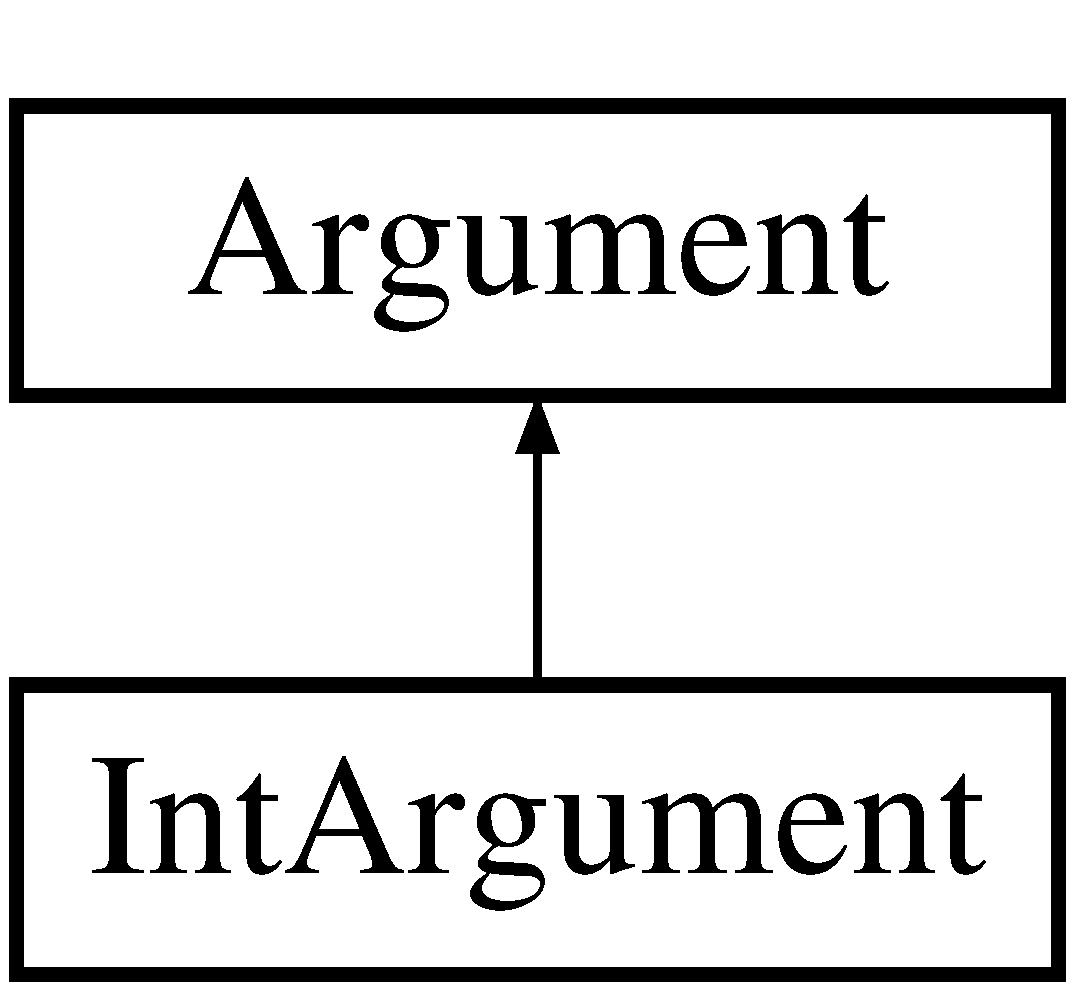
\includegraphics[height=2.000000cm]{classIntArgument}
\end{center}
\end{figure}
\subsection*{Public Member Functions}
\begin{DoxyCompactItemize}
\item 
\hyperlink{classIntArgument_a1ff15a0652a7ed6ef37d8438cac02260}{Int\-Argument} (std\-::string l\-Name, char s\-Name, int $\ast$value, std\-::string descr)
\begin{DoxyCompactList}\small\item\em Constructeur. \end{DoxyCompactList}\item 
int \hyperlink{classIntArgument_af58d4470cb44ed7f383c2cba9ba033e5}{get\-Value} ()
\begin{DoxyCompactList}\small\item\em Accesseur. \end{DoxyCompactList}\item 
void \hyperlink{classIntArgument_ab3a07e2d49a5fba9e79fb0d7585f6a85}{set\-Value} (int val)
\begin{DoxyCompactList}\small\item\em Mutateur. \end{DoxyCompactList}\item 
bool \hyperlink{classIntArgument_a3d27054173466542694fd971b13be8bb}{test\-Value} (std\-::string val)
\begin{DoxyCompactList}\small\item\em Mutateur et testeur. \end{DoxyCompactList}\item 
void \hyperlink{classIntArgument_a8bb885657c1f58c1fbacfc513571ea30}{display} ()
\begin{DoxyCompactList}\small\item\em Afficheur. \end{DoxyCompactList}\item 
\hyperlink{classIntArgument_a700cda557bc17999ef952250f2ba39c6}{$\sim$\-Int\-Argument} ()
\begin{DoxyCompactList}\small\item\em Destructeur. \end{DoxyCompactList}\end{DoxyCompactItemize}


\subsection{Detailed Description}
La classe \hyperlink{classIntArgument}{Int\-Argument} hérite de la classe \hyperlink{classArgument}{Argument}. Les objets de cette classe stockent les informations d'un arguments de type entier, elle posséde une variable qui contient sa valeur (m\-\_\-value). Elle dispose d'un constructeur et des méthodes qui permettent de définir et de tester la valeur d'une instance (\hyperlink{classIntArgument_a3d27054173466542694fd971b13be8bb}{test\-Value()}), d'afficher les informations liées à une instance (\hyperlink{classIntArgument_a8bb885657c1f58c1fbacfc513571ea30}{display()}), d'un accesseur (\hyperlink{classIntArgument_af58d4470cb44ed7f383c2cba9ba033e5}{get\-Value()}) et d'un mutateur (\hyperlink{classIntArgument_ab3a07e2d49a5fba9e79fb0d7585f6a85}{set\-Value(int)}). 

\subsection{Constructor \& Destructor Documentation}
\hypertarget{classIntArgument_a1ff15a0652a7ed6ef37d8438cac02260}{\index{Int\-Argument@{Int\-Argument}!Int\-Argument@{Int\-Argument}}
\index{Int\-Argument@{Int\-Argument}!IntArgument@{Int\-Argument}}
\subsubsection[{Int\-Argument}]{\setlength{\rightskip}{0pt plus 5cm}Int\-Argument\-::\-Int\-Argument (
\begin{DoxyParamCaption}
\item[{std\-::string}]{l\-Name, }
\item[{char}]{s\-Name, }
\item[{int $\ast$}]{value, }
\item[{std\-::string}]{descr}
\end{DoxyParamCaption}
)}}\label{classIntArgument_a1ff15a0652a7ed6ef37d8438cac02260}


Constructeur. 


\begin{DoxyParams}{Parameters}
{\em l\-Name} & \-: Nom long de l'argument \\
\hline
{\em s\-Name} & \-: Nom court de l'argument \\
\hline
{\em value} & \-: Pointeur sur l'entier à modifier \\
\hline
{\em descr} & \-: Description de l'argument\\
\hline
\end{DoxyParams}
Constructeur de la classe \hyperlink{classIntArgument}{Int\-Argument}. \hypertarget{classIntArgument_a700cda557bc17999ef952250f2ba39c6}{\index{Int\-Argument@{Int\-Argument}!$\sim$\-Int\-Argument@{$\sim$\-Int\-Argument}}
\index{$\sim$\-Int\-Argument@{$\sim$\-Int\-Argument}!IntArgument@{Int\-Argument}}
\subsubsection[{$\sim$\-Int\-Argument}]{\setlength{\rightskip}{0pt plus 5cm}Int\-Argument\-::$\sim$\-Int\-Argument (
\begin{DoxyParamCaption}
{}
\end{DoxyParamCaption}
)\hspace{0.3cm}{\ttfamily [inline]}}}\label{classIntArgument_a700cda557bc17999ef952250f2ba39c6}


Destructeur. 

Destructeur de la classe \hyperlink{classIntArgument}{Int\-Argument} 

\subsection{Member Function Documentation}
\hypertarget{classIntArgument_a8bb885657c1f58c1fbacfc513571ea30}{\index{Int\-Argument@{Int\-Argument}!display@{display}}
\index{display@{display}!IntArgument@{Int\-Argument}}
\subsubsection[{display}]{\setlength{\rightskip}{0pt plus 5cm}void Int\-Argument\-::display (
\begin{DoxyParamCaption}
{}
\end{DoxyParamCaption}
)\hspace{0.3cm}{\ttfamily [virtual]}}}\label{classIntArgument_a8bb885657c1f58c1fbacfc513571ea30}


Afficheur. 

C'est une méthode d'affichage d'un argument, l'affichage est sous la forme \-: Int $<$nom$>$ = $<$valeur$>$ 

Implements \hyperlink{classArgument_adab35148c697a617b0b0fcb3169611e3}{Argument}.

\hypertarget{classIntArgument_af58d4470cb44ed7f383c2cba9ba033e5}{\index{Int\-Argument@{Int\-Argument}!get\-Value@{get\-Value}}
\index{get\-Value@{get\-Value}!IntArgument@{Int\-Argument}}
\subsubsection[{get\-Value}]{\setlength{\rightskip}{0pt plus 5cm}int Int\-Argument\-::get\-Value (
\begin{DoxyParamCaption}
{}
\end{DoxyParamCaption}
)\hspace{0.3cm}{\ttfamily [inline]}}}\label{classIntArgument_af58d4470cb44ed7f383c2cba9ba033e5}


Accesseur. 

\begin{DoxyReturn}{Returns}
Valeur de l'\hyperlink{classArgument}{Argument}
\end{DoxyReturn}
Accesseur de m\-\_\-value. \hypertarget{classIntArgument_ab3a07e2d49a5fba9e79fb0d7585f6a85}{\index{Int\-Argument@{Int\-Argument}!set\-Value@{set\-Value}}
\index{set\-Value@{set\-Value}!IntArgument@{Int\-Argument}}
\subsubsection[{set\-Value}]{\setlength{\rightskip}{0pt plus 5cm}void Int\-Argument\-::set\-Value (
\begin{DoxyParamCaption}
\item[{int}]{val}
\end{DoxyParamCaption}
)\hspace{0.3cm}{\ttfamily [inline]}}}\label{classIntArgument_ab3a07e2d49a5fba9e79fb0d7585f6a85}


Mutateur. 


\begin{DoxyParams}{Parameters}
{\em val} & \-: Entier qui donnera sa valeur à la variable m\-\_\-value.\\
\hline
\end{DoxyParams}
Mutateur de m\-\_\-value. \hypertarget{classIntArgument_a3d27054173466542694fd971b13be8bb}{\index{Int\-Argument@{Int\-Argument}!test\-Value@{test\-Value}}
\index{test\-Value@{test\-Value}!IntArgument@{Int\-Argument}}
\subsubsection[{test\-Value}]{\setlength{\rightskip}{0pt plus 5cm}bool Int\-Argument\-::test\-Value (
\begin{DoxyParamCaption}
\item[{std\-::string}]{val}
\end{DoxyParamCaption}
)\hspace{0.3cm}{\ttfamily [virtual]}}}\label{classIntArgument_a3d27054173466542694fd971b13be8bb}


Mutateur et testeur. 


\begin{DoxyParams}{Parameters}
{\em val} & \-: valeur de l'argument \\
\hline
\end{DoxyParams}
\begin{DoxyReturn}{Returns}
Vrai si la valeur est du bon type, faux sinon. C'est une méthode qui prend en paramètre la valeur d'un argument via la ligne de commande et qui test si elle correspond bien à un entier. Si c'est le cas, la méthode met la valeur dans l'instance et retourne vrai, sinon faux. 
\end{DoxyReturn}


Implements \hyperlink{classArgument_a20b6a0182f1402dd36b20b1a6743e665}{Argument}.



The documentation for this class was generated from the following files\-:\begin{DoxyCompactItemize}
\item 
src/\hyperlink{IntArgument_8h}{Int\-Argument.\-h}\item 
src/\hyperlink{IntArgument_8cpp}{Int\-Argument.\-cpp}\end{DoxyCompactItemize}

\hypertarget{classUnsignedIntArgument}{\section{Unsigned\-Int\-Argument Class Reference}
\label{classUnsignedIntArgument}\index{Unsigned\-Int\-Argument@{Unsigned\-Int\-Argument}}
}


{\ttfamily \#include $<$Unsigned\-Int\-Argument.\-h$>$}

Inheritance diagram for Unsigned\-Int\-Argument\-:\begin{figure}[H]
\begin{center}
\leavevmode
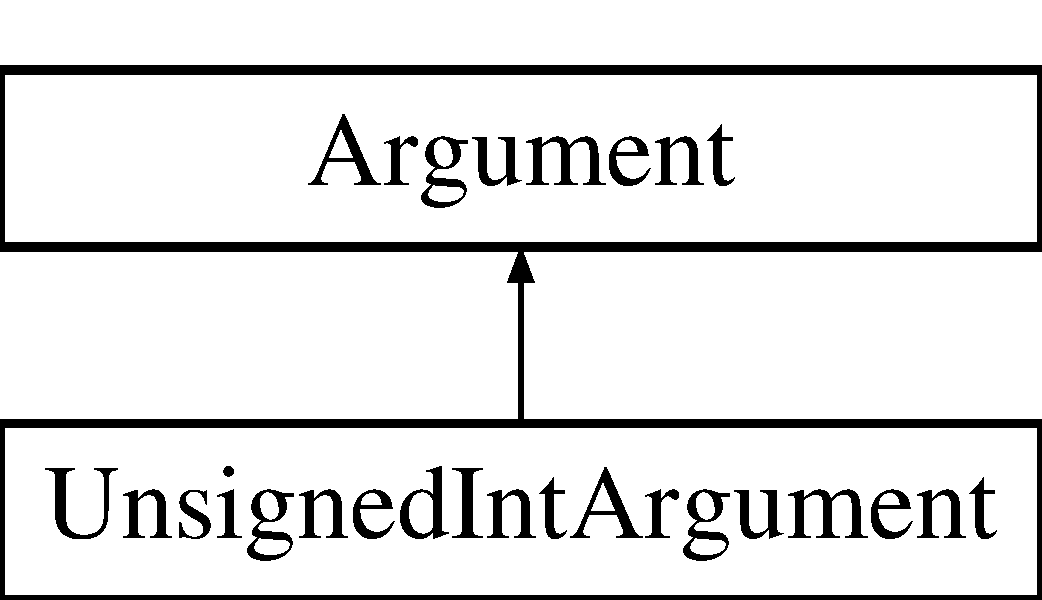
\includegraphics[height=2.000000cm]{classUnsignedIntArgument}
\end{center}
\end{figure}
\subsection*{Public Member Functions}
\begin{DoxyCompactItemize}
\item 
\hyperlink{classUnsignedIntArgument_a6254cd2a6fd9df7294a5c267ea11ffb0}{Unsigned\-Int\-Argument} (std\-::string l\-Name, char s\-Name, unsigned int $\ast$value, std\-::string descr)
\begin{DoxyCompactList}\small\item\em Constructeur. \end{DoxyCompactList}\item 
unsigned int \hyperlink{classUnsignedIntArgument_ab4dff7bc225b9313437ed45a1debddf6}{get\-Value} ()
\begin{DoxyCompactList}\small\item\em Accesseur. \end{DoxyCompactList}\item 
void \hyperlink{classUnsignedIntArgument_aa5c187eb0c69d2ab0148ab7b780ecf70}{set\-Value} (unsigned int val)
\begin{DoxyCompactList}\small\item\em Mutateur. \end{DoxyCompactList}\item 
bool \hyperlink{classUnsignedIntArgument_a46d930be372e3443fc3f3a2419ceb387}{test\-Value} (std\-::string val)
\begin{DoxyCompactList}\small\item\em Mutateur et testeur. \end{DoxyCompactList}\item 
void \hyperlink{classUnsignedIntArgument_a4abf29719479c55ee030821e02699834}{display} ()
\begin{DoxyCompactList}\small\item\em Afficheur. \end{DoxyCompactList}\item 
\hyperlink{classUnsignedIntArgument_a7cceb33cfeae1fe3274c3e08d6636fe1}{$\sim$\-Unsigned\-Int\-Argument} ()
\begin{DoxyCompactList}\small\item\em Destructeur. \end{DoxyCompactList}\end{DoxyCompactItemize}


\subsection{Detailed Description}
La classe \hyperlink{classUnsignedIntArgument}{Unsigned\-Int\-Argument} hérite de la classe \hyperlink{classArgument}{Argument}. Les objets de cette classe stockent les informations d'un arguments de type unsigned int, elle possède une variable qui contient sa valeur (m\-\_\-value). Elle dispose d'un constructeur et des méthodes qui permettent de définir et de tester la valeur d'une instance (\hyperlink{classUnsignedIntArgument_a46d930be372e3443fc3f3a2419ceb387}{test\-Value()}), d'afficher les informations liées à une instance (\hyperlink{classUnsignedIntArgument_a4abf29719479c55ee030821e02699834}{display()}), d'un accesseur (\hyperlink{classUnsignedIntArgument_ab4dff7bc225b9313437ed45a1debddf6}{get\-Value()}) et d'un mutateur (\hyperlink{classUnsignedIntArgument_aa5c187eb0c69d2ab0148ab7b780ecf70}{set\-Value(unsigned int)}). 

\subsection{Constructor \& Destructor Documentation}
\hypertarget{classUnsignedIntArgument_a6254cd2a6fd9df7294a5c267ea11ffb0}{\index{Unsigned\-Int\-Argument@{Unsigned\-Int\-Argument}!Unsigned\-Int\-Argument@{Unsigned\-Int\-Argument}}
\index{Unsigned\-Int\-Argument@{Unsigned\-Int\-Argument}!UnsignedIntArgument@{Unsigned\-Int\-Argument}}
\subsubsection[{Unsigned\-Int\-Argument}]{\setlength{\rightskip}{0pt plus 5cm}Unsigned\-Int\-Argument\-::\-Unsigned\-Int\-Argument (
\begin{DoxyParamCaption}
\item[{std\-::string}]{l\-Name, }
\item[{char}]{s\-Name, }
\item[{unsigned int $\ast$}]{value, }
\item[{std\-::string}]{descr}
\end{DoxyParamCaption}
)}}\label{classUnsignedIntArgument_a6254cd2a6fd9df7294a5c267ea11ffb0}


Constructeur. 


\begin{DoxyParams}{Parameters}
{\em l\-Name} & \-: Nom long de l'argument \\
\hline
{\em s\-Name} & \-: Nom court de l'argument \\
\hline
{\em value} & \-: Pointeur sur l'unsigned int à modifier \\
\hline
{\em descr} & \-: Description de l'argument\\
\hline
\end{DoxyParams}
Constructeur de la classe \hyperlink{classUnsignedIntArgument}{Unsigned\-Int\-Argument}. \hypertarget{classUnsignedIntArgument_a7cceb33cfeae1fe3274c3e08d6636fe1}{\index{Unsigned\-Int\-Argument@{Unsigned\-Int\-Argument}!$\sim$\-Unsigned\-Int\-Argument@{$\sim$\-Unsigned\-Int\-Argument}}
\index{$\sim$\-Unsigned\-Int\-Argument@{$\sim$\-Unsigned\-Int\-Argument}!UnsignedIntArgument@{Unsigned\-Int\-Argument}}
\subsubsection[{$\sim$\-Unsigned\-Int\-Argument}]{\setlength{\rightskip}{0pt plus 5cm}Unsigned\-Int\-Argument\-::$\sim$\-Unsigned\-Int\-Argument (
\begin{DoxyParamCaption}
{}
\end{DoxyParamCaption}
)\hspace{0.3cm}{\ttfamily [inline]}}}\label{classUnsignedIntArgument_a7cceb33cfeae1fe3274c3e08d6636fe1}


Destructeur. 

Destructeur de la classe \hyperlink{classUnsignedIntArgument}{Unsigned\-Int\-Argument} 

\subsection{Member Function Documentation}
\hypertarget{classUnsignedIntArgument_a4abf29719479c55ee030821e02699834}{\index{Unsigned\-Int\-Argument@{Unsigned\-Int\-Argument}!display@{display}}
\index{display@{display}!UnsignedIntArgument@{Unsigned\-Int\-Argument}}
\subsubsection[{display}]{\setlength{\rightskip}{0pt plus 5cm}void Unsigned\-Int\-Argument\-::display (
\begin{DoxyParamCaption}
{}
\end{DoxyParamCaption}
)\hspace{0.3cm}{\ttfamily [virtual]}}}\label{classUnsignedIntArgument_a4abf29719479c55ee030821e02699834}


Afficheur. 

C'est une méthode d'affichage d'un argument, l'affichage est sous la forme \-: Unsigned int $<$nom$>$ = $<$valeur$>$ 

Implements \hyperlink{classArgument_adab35148c697a617b0b0fcb3169611e3}{Argument}.

\hypertarget{classUnsignedIntArgument_ab4dff7bc225b9313437ed45a1debddf6}{\index{Unsigned\-Int\-Argument@{Unsigned\-Int\-Argument}!get\-Value@{get\-Value}}
\index{get\-Value@{get\-Value}!UnsignedIntArgument@{Unsigned\-Int\-Argument}}
\subsubsection[{get\-Value}]{\setlength{\rightskip}{0pt plus 5cm}bool Unsigned\-Int\-Argument\-::get\-Value (
\begin{DoxyParamCaption}
{}
\end{DoxyParamCaption}
)\hspace{0.3cm}{\ttfamily [inline]}}}\label{classUnsignedIntArgument_ab4dff7bc225b9313437ed45a1debddf6}


Accesseur. 

\begin{DoxyReturn}{Returns}
Valeur de l'argument
\end{DoxyReturn}
Accesseur de m\-\_\-value. \hypertarget{classUnsignedIntArgument_aa5c187eb0c69d2ab0148ab7b780ecf70}{\index{Unsigned\-Int\-Argument@{Unsigned\-Int\-Argument}!set\-Value@{set\-Value}}
\index{set\-Value@{set\-Value}!UnsignedIntArgument@{Unsigned\-Int\-Argument}}
\subsubsection[{set\-Value}]{\setlength{\rightskip}{0pt plus 5cm}void Unsigned\-Int\-Argument\-::set\-Value (
\begin{DoxyParamCaption}
\item[{unsigned int}]{val}
\end{DoxyParamCaption}
)\hspace{0.3cm}{\ttfamily [inline]}}}\label{classUnsignedIntArgument_aa5c187eb0c69d2ab0148ab7b780ecf70}


Mutateur. 


\begin{DoxyParams}{Parameters}
{\em val} & \-: Entier qui donnera sa valeur à la variable m\-\_\-value.\\
\hline
\end{DoxyParams}
Mutateur de m\-\_\-value. \hypertarget{classUnsignedIntArgument_a46d930be372e3443fc3f3a2419ceb387}{\index{Unsigned\-Int\-Argument@{Unsigned\-Int\-Argument}!test\-Value@{test\-Value}}
\index{test\-Value@{test\-Value}!UnsignedIntArgument@{Unsigned\-Int\-Argument}}
\subsubsection[{test\-Value}]{\setlength{\rightskip}{0pt plus 5cm}bool Unsigned\-Int\-Argument\-::test\-Value (
\begin{DoxyParamCaption}
\item[{std\-::string}]{val}
\end{DoxyParamCaption}
)\hspace{0.3cm}{\ttfamily [virtual]}}}\label{classUnsignedIntArgument_a46d930be372e3443fc3f3a2419ceb387}


Mutateur et testeur. 


\begin{DoxyParams}{Parameters}
{\em val} & \-: valeur d'un argument \\
\hline
\end{DoxyParams}
\begin{DoxyReturn}{Returns}
Vrai si la valeur est du bon type, faux sinon.
\end{DoxyReturn}
C'est une méthode qui prend en paramètre la valeur d'un argument via la ligne de commande et qui test si elle correspond bien à un unsigned int. Si c'est le cas, la méthode met la valeur dans l'instance et retourne vrai, sinon faux. 

Implements \hyperlink{classArgument_a20b6a0182f1402dd36b20b1a6743e665}{Argument}.



The documentation for this class was generated from the following files\-:\begin{DoxyCompactItemize}
\item 
src/\hyperlink{UnsignedIntArgument_8h}{Unsigned\-Int\-Argument.\-h}\item 
src/\hyperlink{UnsignedIntArgument_8cpp}{Unsigned\-Int\-Argument.\-cpp}\end{DoxyCompactItemize}

\hypertarget{classVecArgument}{\section{Vec\-Argument Class Reference}
\label{classVecArgument}\index{Vec\-Argument@{Vec\-Argument}}
}


{\ttfamily \#include $<$Vec\-Argument.\-h$>$}

Inheritance diagram for Vec\-Argument\-:\begin{figure}[H]
\begin{center}
\leavevmode
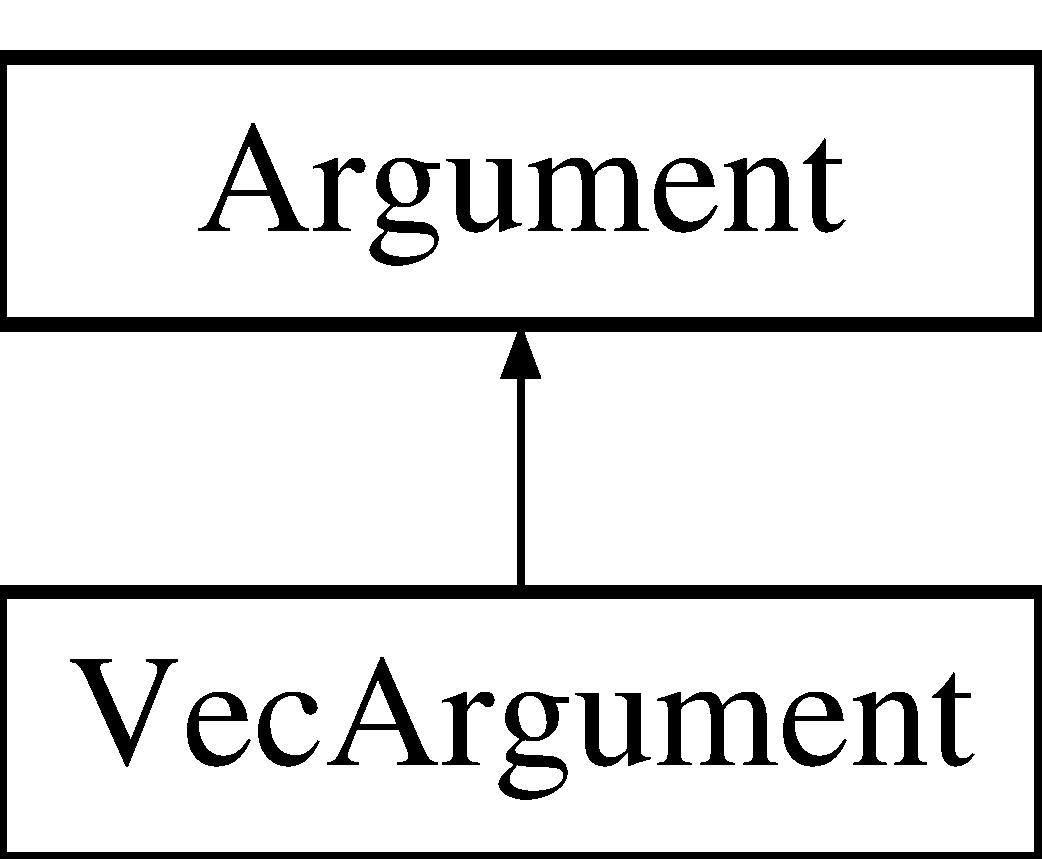
\includegraphics[height=2.000000cm]{classVecArgument}
\end{center}
\end{figure}
\subsection*{Public Member Functions}
\begin{DoxyCompactItemize}
\item 
\hyperlink{classVecArgument_aec430730db7a84e0529c4385b60406d7}{Vec\-Argument} (std\-::string l\-Name, char s\-Name, std\-::string $\ast$value, std\-::vector$<$ std\-::string $>$ vec, std\-::string descr)
\begin{DoxyCompactList}\small\item\em Constructeur. \end{DoxyCompactList}\item 
std\-::string \hyperlink{classVecArgument_a45634f1256decb5aed723b9da11db7ad}{get\-Value} ()
\begin{DoxyCompactList}\small\item\em Accesseur. \end{DoxyCompactList}\item 
void \hyperlink{classVecArgument_ab83b7cf9a619de8086743017debee409}{set\-Value} (std\-::string val)
\begin{DoxyCompactList}\small\item\em Mutateur. \end{DoxyCompactList}\item 
bool \hyperlink{classVecArgument_a2b3cbbc68d03d2eec8dd00452d228ef1}{test\-Value} (std\-::string val)
\begin{DoxyCompactList}\small\item\em Mutateur et testeurstring$>$ Vec\-Argument\-::get. \end{DoxyCompactList}\item 
void \hyperlink{classVecArgument_ae3611e8947ccbd26681044f20df4b351}{display} ()
\begin{DoxyCompactList}\small\item\em Afficheur. \end{DoxyCompactList}\item 
\hyperlink{classVecArgument_ae4dbf015d767e2501434c63577f4a30b}{$\sim$\-Vec\-Argument} ()
\begin{DoxyCompactList}\small\item\em Destructeur. \end{DoxyCompactList}\item 
std\-::vector$<$ std\-::string $>$ \hyperlink{classVecArgument_ac9d4c2a47cb82df6a2d3791349c9aa56}{get\-Vect} ()
\begin{DoxyCompactList}\small\item\em Accesseur. \end{DoxyCompactList}\end{DoxyCompactItemize}


\subsection{Detailed Description}
La classe \hyperlink{classVecArgument}{Vec\-Argument} hérite de la classe \hyperlink{classArgument}{Argument}. Les objets de cette classe stockent les informations d'un arguments de type vecteur, elle possède une variable qui contient sa valeur (m\-\_\-value) et une autre qui contient le vecteur de choix (m\-\_\-vec\-Str). Elle dispose d'un constructeur et des méthodes qui permettent de définir et de tester la valeur d'une instance (\hyperlink{classVecArgument_a2b3cbbc68d03d2eec8dd00452d228ef1}{test\-Value()}), d'afficher les informations liées à une instance (\hyperlink{classVecArgument_ae3611e8947ccbd26681044f20df4b351}{display()}), d'un accesseur (\hyperlink{classVecArgument_a45634f1256decb5aed723b9da11db7ad}{get\-Value()}) et d'un mutateur (\hyperlink{classVecArgument_ab83b7cf9a619de8086743017debee409}{set\-Value(std\-::string)}). 

\subsection{Constructor \& Destructor Documentation}
\hypertarget{classVecArgument_aec430730db7a84e0529c4385b60406d7}{\index{Vec\-Argument@{Vec\-Argument}!Vec\-Argument@{Vec\-Argument}}
\index{Vec\-Argument@{Vec\-Argument}!VecArgument@{Vec\-Argument}}
\subsubsection[{Vec\-Argument}]{\setlength{\rightskip}{0pt plus 5cm}Vec\-Argument\-::\-Vec\-Argument (
\begin{DoxyParamCaption}
\item[{std\-::string}]{l\-Name, }
\item[{char}]{s\-Name, }
\item[{std\-::string $\ast$}]{value, }
\item[{std\-::vector$<$ std\-::string $>$}]{vec, }
\item[{std\-::string}]{descr}
\end{DoxyParamCaption}
)}}\label{classVecArgument_aec430730db7a84e0529c4385b60406d7}


Constructeur. 


\begin{DoxyParams}{Parameters}
{\em l\-Name} & \-: Nom long de l'argument \\
\hline
{\em s\-Name} & \-: Nom court de l'argument \\
\hline
{\em value} & \-: Pointeur sur la chaîne de caractères à modifier \\
\hline
{\em vec} & \-: Vecteur de chaîne de caractères des choix possibles \\
\hline
{\em descr} & \-: Description de l'argument\\
\hline
\end{DoxyParams}
Constructeur de la classe \hyperlink{classVecArgument}{Vec\-Argument}. \hypertarget{classVecArgument_ae4dbf015d767e2501434c63577f4a30b}{\index{Vec\-Argument@{Vec\-Argument}!$\sim$\-Vec\-Argument@{$\sim$\-Vec\-Argument}}
\index{$\sim$\-Vec\-Argument@{$\sim$\-Vec\-Argument}!VecArgument@{Vec\-Argument}}
\subsubsection[{$\sim$\-Vec\-Argument}]{\setlength{\rightskip}{0pt plus 5cm}Vec\-Argument\-::$\sim$\-Vec\-Argument (
\begin{DoxyParamCaption}
{}
\end{DoxyParamCaption}
)\hspace{0.3cm}{\ttfamily [inline]}}}\label{classVecArgument_ae4dbf015d767e2501434c63577f4a30b}


Destructeur. 

Destructeur de la classe \hyperlink{classVecArgument}{Vec\-Argument} 

\subsection{Member Function Documentation}
\hypertarget{classVecArgument_ae3611e8947ccbd26681044f20df4b351}{\index{Vec\-Argument@{Vec\-Argument}!display@{display}}
\index{display@{display}!VecArgument@{Vec\-Argument}}
\subsubsection[{display}]{\setlength{\rightskip}{0pt plus 5cm}void Vec\-Argument\-::display (
\begin{DoxyParamCaption}
{}
\end{DoxyParamCaption}
)\hspace{0.3cm}{\ttfamily [virtual]}}}\label{classVecArgument_ae3611e8947ccbd26681044f20df4b351}


Afficheur. 

C'est une méthode d'affichage d'un argument, l'affichage est sous la forme \-: Tab $<$nom$>$ = $<$valeur$>$ 

Implements \hyperlink{classArgument_adab35148c697a617b0b0fcb3169611e3}{Argument}.

\hypertarget{classVecArgument_a45634f1256decb5aed723b9da11db7ad}{\index{Vec\-Argument@{Vec\-Argument}!get\-Value@{get\-Value}}
\index{get\-Value@{get\-Value}!VecArgument@{Vec\-Argument}}
\subsubsection[{get\-Value}]{\setlength{\rightskip}{0pt plus 5cm}bool Vec\-Argument\-::get\-Value (
\begin{DoxyParamCaption}
{}
\end{DoxyParamCaption}
)\hspace{0.3cm}{\ttfamily [inline]}}}\label{classVecArgument_a45634f1256decb5aed723b9da11db7ad}


Accesseur. 

\begin{DoxyReturn}{Returns}
Valeur de l'argument
\end{DoxyReturn}
Accesseur de m\-\_\-value. \hypertarget{classVecArgument_ac9d4c2a47cb82df6a2d3791349c9aa56}{\index{Vec\-Argument@{Vec\-Argument}!get\-Vect@{get\-Vect}}
\index{get\-Vect@{get\-Vect}!VecArgument@{Vec\-Argument}}
\subsubsection[{get\-Vect}]{\setlength{\rightskip}{0pt plus 5cm}vector$<$ string $>$ Vec\-Argument\-::get\-Vect (
\begin{DoxyParamCaption}
{}
\end{DoxyParamCaption}
)}}\label{classVecArgument_ac9d4c2a47cb82df6a2d3791349c9aa56}


Accesseur. 

\begin{DoxyReturn}{Returns}
Le vecteur de valeur en chaîne de caractère
\end{DoxyReturn}
Accesseur de m\-\_\-vec\-Str \hypertarget{classVecArgument_ab83b7cf9a619de8086743017debee409}{\index{Vec\-Argument@{Vec\-Argument}!set\-Value@{set\-Value}}
\index{set\-Value@{set\-Value}!VecArgument@{Vec\-Argument}}
\subsubsection[{set\-Value}]{\setlength{\rightskip}{0pt plus 5cm}void Vec\-Argument\-::set\-Value (
\begin{DoxyParamCaption}
\item[{std\-::string}]{val}
\end{DoxyParamCaption}
)\hspace{0.3cm}{\ttfamily [inline]}}}\label{classVecArgument_ab83b7cf9a619de8086743017debee409}


Mutateur. 


\begin{DoxyParams}{Parameters}
{\em val} & \-: Chaîne de caractère qui donnera sa valeur à la variable m\-\_\-value.\\
\hline
\end{DoxyParams}
Mutateur de m\-\_\-value. \hypertarget{classVecArgument_a2b3cbbc68d03d2eec8dd00452d228ef1}{\index{Vec\-Argument@{Vec\-Argument}!test\-Value@{test\-Value}}
\index{test\-Value@{test\-Value}!VecArgument@{Vec\-Argument}}
\subsubsection[{test\-Value}]{\setlength{\rightskip}{0pt plus 5cm}bool Vec\-Argument\-::test\-Value (
\begin{DoxyParamCaption}
\item[{std\-::string}]{val}
\end{DoxyParamCaption}
)\hspace{0.3cm}{\ttfamily [virtual]}}}\label{classVecArgument_a2b3cbbc68d03d2eec8dd00452d228ef1}


Mutateur et testeurstring$>$ Vec\-Argument\-::get. 


\begin{DoxyParams}{Parameters}
{\em val} & \-: valeur d'un argument \\
\hline
\end{DoxyParams}
\begin{DoxyReturn}{Returns}
Vrai si la valeur est du bon type, faux sinon.
\end{DoxyReturn}
C'est une méthode qui prend en paramètre la valeur d'un argument via la ligne de commande et qui test si elle est bien incluse dans le vecteur de l'instance. Si c'est le cas, la méthode met la valeur dans l'instance et retourne vrai, sinon faux. 

Implements \hyperlink{classArgument_a20b6a0182f1402dd36b20b1a6743e665}{Argument}.



The documentation for this class was generated from the following files\-:\begin{DoxyCompactItemize}
\item 
src/\hyperlink{VecArgument_8h}{Vec\-Argument.\-h}\item 
src/\hyperlink{VecArgument_8cpp}{Vec\-Argument.\-cpp}\end{DoxyCompactItemize}

\chapter{File Documentation}
\hypertarget{Argument_8cpp}{\section{src/\-Argument.cpp File Reference}
\label{Argument_8cpp}\index{src/\-Argument.\-cpp@{src/\-Argument.\-cpp}}
}


Code C++ de la classe \hyperlink{classArgument}{Argument}.  


{\ttfamily \#include \char`\"{}Argument.\-h\char`\"{}}\\*
{\ttfamily \#include $<$string.\-h$>$}\\*
\subsection*{Macros}
\begin{DoxyCompactItemize}
\item 
\hypertarget{Argument_8cpp_aefa1812986b72006dfd696758098abe7}{\#define {\bfseries underline}~\char`\"{}\textbackslash{}33\mbox{[}4m\char`\"{}}\label{Argument_8cpp_aefa1812986b72006dfd696758098abe7}

\item 
\hypertarget{Argument_8cpp_a913bd037bde194a64444f401f6c2b215}{\#define {\bfseries end\-\_\-underline}~\char`\"{}\textbackslash{}033\mbox{[}0m\char`\"{}}\label{Argument_8cpp_a913bd037bde194a64444f401f6c2b215}

\item 
\hypertarget{Argument_8cpp_a530f00c8dc2d1aaefe8a048b417e7290}{\#define {\bfseries bold}~\char`\"{}\textbackslash{}033\mbox{[}1m\char`\"{}}\label{Argument_8cpp_a530f00c8dc2d1aaefe8a048b417e7290}

\item 
\hypertarget{Argument_8cpp_ab6f843fa435bc9d997df99f8bfc45863}{\#define {\bfseries end\-\_\-bold}~\char`\"{}\textbackslash{}033\mbox{[}0m\char`\"{}}\label{Argument_8cpp_ab6f843fa435bc9d997df99f8bfc45863}

\end{DoxyCompactItemize}


\subsection{Detailed Description}
Code C++ de la classe \hyperlink{classArgument}{Argument}. \begin{DoxyAuthor}{Author}
\{ Valérian De Leeuw, Robin Couasnet \} 
\end{DoxyAuthor}
\begin{DoxyDate}{Date}
20 avril 2015 
\end{DoxyDate}

\hypertarget{Argument_8h}{\section{src/\-Argument.h File Reference}
\label{Argument_8h}\index{src/\-Argument.\-h@{src/\-Argument.\-h}}
}


Header de la classe \hyperlink{classArgument}{Argument}.  


{\ttfamily \#include $<$iostream$>$}\\*
\subsection*{Classes}
\begin{DoxyCompactItemize}
\item 
class \hyperlink{classArgument}{Argument}
\end{DoxyCompactItemize}


\subsection{Detailed Description}
Header de la classe \hyperlink{classArgument}{Argument}. \begin{DoxyAuthor}{Author}
\{ Valérian De Leeuw, Robin Couasnet \} 
\end{DoxyAuthor}
\begin{DoxyDate}{Date}
20 avril 2015 
\end{DoxyDate}

\hypertarget{BoolArgument_8cpp}{\section{src/\-Bool\-Argument.cpp File Reference}
\label{BoolArgument_8cpp}\index{src/\-Bool\-Argument.\-cpp@{src/\-Bool\-Argument.\-cpp}}
}


Code C++ de la classe \hyperlink{classBoolArgument}{Bool\-Argument}.  


{\ttfamily \#include \char`\"{}Bool\-Argument.\-h\char`\"{}}\\*
{\ttfamily \#include $<$boost/lexical\-\_\-cast.\-hpp$>$}\\*
{\ttfamily \#include $<$string.\-h$>$}\\*


\subsection{Detailed Description}
Code C++ de la classe \hyperlink{classBoolArgument}{Bool\-Argument}. \begin{DoxyAuthor}{Author}
\{ Valérian De Leeuw, Robin Couasnet \} 
\end{DoxyAuthor}
\begin{DoxyDate}{Date}
20 avril 2015 
\end{DoxyDate}

\hypertarget{BoolArgument_8h}{\section{src/\-Bool\-Argument.h File Reference}
\label{BoolArgument_8h}\index{src/\-Bool\-Argument.\-h@{src/\-Bool\-Argument.\-h}}
}


Header de la classe \hyperlink{classBoolArgument}{Bool\-Argument}.  


{\ttfamily \#include \char`\"{}Argument.\-h\char`\"{}}\\*
\subsection*{Classes}
\begin{DoxyCompactItemize}
\item 
class \hyperlink{classBoolArgument}{Bool\-Argument}
\end{DoxyCompactItemize}


\subsection{Detailed Description}
Header de la classe \hyperlink{classBoolArgument}{Bool\-Argument}. \begin{DoxyAuthor}{Author}
\{ Valérian De Leeuw, Robin Couasnet \} 
\end{DoxyAuthor}
\begin{DoxyDate}{Date}
20 avril 2015 
\end{DoxyDate}

\hypertarget{CommandLine_8cpp}{\section{src/\-Command\-Line.cpp File Reference}
\label{CommandLine_8cpp}\index{src/\-Command\-Line.\-cpp@{src/\-Command\-Line.\-cpp}}
}


Code C++ de la classe \hyperlink{classCommandLine}{Command\-Line}.  


{\ttfamily \#include \char`\"{}Command\-Line.\-h\char`\"{}}\\*
{\ttfamily \#include $<$sstream$>$}\\*
{\ttfamily \#include $<$iostream$>$}\\*
{\ttfamily \#include $<$string$>$}\\*
{\ttfamily \#include $<$string.\-h$>$}\\*
{\ttfamily \#include $<$stdexcept$>$}\\*
{\ttfamily \#include $<$typeinfo$>$}\\*
\subsection*{Macros}
\begin{DoxyCompactItemize}
\item 
\hypertarget{CommandLine_8cpp_aefa1812986b72006dfd696758098abe7}{\#define {\bfseries underline}~\char`\"{}\textbackslash{}33\mbox{[}4m\char`\"{}}\label{CommandLine_8cpp_aefa1812986b72006dfd696758098abe7}

\item 
\hypertarget{CommandLine_8cpp_a913bd037bde194a64444f401f6c2b215}{\#define {\bfseries end\-\_\-underline}~\char`\"{}\textbackslash{}033\mbox{[}0m\char`\"{}}\label{CommandLine_8cpp_a913bd037bde194a64444f401f6c2b215}

\item 
\hypertarget{CommandLine_8cpp_a530f00c8dc2d1aaefe8a048b417e7290}{\#define {\bfseries bold}~\char`\"{}\textbackslash{}033\mbox{[}1m\char`\"{}}\label{CommandLine_8cpp_a530f00c8dc2d1aaefe8a048b417e7290}

\item 
\hypertarget{CommandLine_8cpp_ab6f843fa435bc9d997df99f8bfc45863}{\#define {\bfseries end\-\_\-bold}~\char`\"{}\textbackslash{}033\mbox{[}0m\char`\"{}}\label{CommandLine_8cpp_ab6f843fa435bc9d997df99f8bfc45863}

\end{DoxyCompactItemize}


\subsection{Detailed Description}
Code C++ de la classe \hyperlink{classCommandLine}{Command\-Line}. \begin{DoxyAuthor}{Author}
\{ Valérian De Leeuw, Robin Couasnet \} 
\end{DoxyAuthor}
\begin{DoxyDate}{Date}
20 avril 2015 
\end{DoxyDate}

\hypertarget{CommandLine_8h}{\section{src/\-Command\-Line.h File Reference}
\label{CommandLine_8h}\index{src/\-Command\-Line.\-h@{src/\-Command\-Line.\-h}}
}


Header de la classe \hyperlink{classCommandLine}{Command\-Line}.  


{\ttfamily \#include \char`\"{}Argument.\-h\char`\"{}}\\*
{\ttfamily \#include \char`\"{}Int\-Argument.\-h\char`\"{}}\\*
{\ttfamily \#include \char`\"{}Unsigned\-Int\-Argument.\-h\char`\"{}}\\*
{\ttfamily \#include \char`\"{}Float\-Argument.\-h\char`\"{}}\\*
{\ttfamily \#include \char`\"{}Bool\-Argument.\-h\char`\"{}}\\*
{\ttfamily \#include \char`\"{}Vec\-Argument.\-h\char`\"{}}\\*
{\ttfamily \#include \char`\"{}Flag\-Argument.\-h\char`\"{}}\\*
{\ttfamily \#include $<$vector$>$}\\*
\subsection*{Classes}
\begin{DoxyCompactItemize}
\item 
class \hyperlink{classCommandLine}{Command\-Line}
\end{DoxyCompactItemize}


\subsection{Detailed Description}
Header de la classe \hyperlink{classCommandLine}{Command\-Line}. \begin{DoxyAuthor}{Author}
\{ Valérian De Leeuw, Robin Couasnet \} 
\end{DoxyAuthor}
\begin{DoxyDate}{Date}
20 avril 2015 
\end{DoxyDate}

\hypertarget{FlagArgument_8cpp}{\section{src/\-Flag\-Argument.cpp File Reference}
\label{FlagArgument_8cpp}\index{src/\-Flag\-Argument.\-cpp@{src/\-Flag\-Argument.\-cpp}}
}


Code C++ de la classe \hyperlink{classFlagArgument}{Flag\-Argument}.  


{\ttfamily \#include \char`\"{}Flag\-Argument.\-h\char`\"{}}\\*
{\ttfamily \#include $<$boost/lexical\-\_\-cast.\-hpp$>$}\\*
{\ttfamily \#include $<$string.\-h$>$}\\*


\subsection{Detailed Description}
Code C++ de la classe \hyperlink{classFlagArgument}{Flag\-Argument}. \begin{DoxyAuthor}{Author}
\{ Valérian De Leeuw, Robin Couasnet \} 
\end{DoxyAuthor}
\begin{DoxyDate}{Date}
27 avril 2015 
\end{DoxyDate}

\hypertarget{FlagArgument_8h}{\section{src/\-Flag\-Argument.h File Reference}
\label{FlagArgument_8h}\index{src/\-Flag\-Argument.\-h@{src/\-Flag\-Argument.\-h}}
}


Header de la classe \hyperlink{classFlagArgument}{Flag\-Argument}.  


{\ttfamily \#include \char`\"{}Argument.\-h\char`\"{}}\\*
\subsection*{Classes}
\begin{DoxyCompactItemize}
\item 
class \hyperlink{classFlagArgument}{Flag\-Argument}
\end{DoxyCompactItemize}


\subsection{Detailed Description}
Header de la classe \hyperlink{classFlagArgument}{Flag\-Argument}. \begin{DoxyAuthor}{Author}
\{ Valérian De Leeuw, Robin Couasnet \} 
\end{DoxyAuthor}
\begin{DoxyDate}{Date}
27 avril 2015 
\end{DoxyDate}

\hypertarget{FloatArgument_8cpp}{\section{src/\-Float\-Argument.cpp File Reference}
\label{FloatArgument_8cpp}\index{src/\-Float\-Argument.\-cpp@{src/\-Float\-Argument.\-cpp}}
}


Code C++ de la classe \hyperlink{classFloatArgument}{Float\-Argument}.  


{\ttfamily \#include \char`\"{}Float\-Argument.\-h\char`\"{}}\\*
{\ttfamily \#include $<$boost/lexical\-\_\-cast.\-hpp$>$}\\*
{\ttfamily \#include $<$string.\-h$>$}\\*


\subsection{Detailed Description}
Code C++ de la classe \hyperlink{classFloatArgument}{Float\-Argument}. \begin{DoxyAuthor}{Author}
\{ Valérian De Leeuw, Robin Couasnet \} 
\end{DoxyAuthor}
\begin{DoxyDate}{Date}
20 avril 2015 
\end{DoxyDate}

\hypertarget{FloatArgument_8h}{\section{src/\-Float\-Argument.h File Reference}
\label{FloatArgument_8h}\index{src/\-Float\-Argument.\-h@{src/\-Float\-Argument.\-h}}
}


Header de la classe \hyperlink{classFloatArgument}{Float\-Argument}.  


{\ttfamily \#include \char`\"{}Argument.\-h\char`\"{}}\\*
\subsection*{Classes}
\begin{DoxyCompactItemize}
\item 
class \hyperlink{classFloatArgument}{Float\-Argument}
\end{DoxyCompactItemize}


\subsection{Detailed Description}
Header de la classe \hyperlink{classFloatArgument}{Float\-Argument}. \begin{DoxyAuthor}{Author}
\{ Valérian De Leeuw, Robin Couasnet \} 
\end{DoxyAuthor}
\begin{DoxyDate}{Date}
20 avril 2015 
\end{DoxyDate}

\hypertarget{IntArgument_8cpp}{\section{src/\-Int\-Argument.cpp File Reference}
\label{IntArgument_8cpp}\index{src/\-Int\-Argument.\-cpp@{src/\-Int\-Argument.\-cpp}}
}


Code C++ de la classe \hyperlink{classIntArgument}{Int\-Argument}.  


{\ttfamily \#include \char`\"{}Int\-Argument.\-h\char`\"{}}\\*
{\ttfamily \#include $<$boost/lexical\-\_\-cast.\-hpp$>$}\\*
{\ttfamily \#include $<$string.\-h$>$}\\*


\subsection{Detailed Description}
Code C++ de la classe \hyperlink{classIntArgument}{Int\-Argument}. \begin{DoxyAuthor}{Author}
\{ Valérian De Leeuw, Robin Couasnet \} 
\end{DoxyAuthor}
\begin{DoxyDate}{Date}
20 avril 2015 
\end{DoxyDate}

\hypertarget{IntArgument_8h}{\section{src/\-Int\-Argument.h File Reference}
\label{IntArgument_8h}\index{src/\-Int\-Argument.\-h@{src/\-Int\-Argument.\-h}}
}


Header de la classe \hyperlink{classIntArgument}{Int\-Argument}.  


{\ttfamily \#include \char`\"{}Argument.\-h\char`\"{}}\\*
\subsection*{Classes}
\begin{DoxyCompactItemize}
\item 
class \hyperlink{classIntArgument}{Int\-Argument}
\end{DoxyCompactItemize}


\subsection{Detailed Description}
Header de la classe \hyperlink{classIntArgument}{Int\-Argument}. \begin{DoxyAuthor}{Author}
\{ Valérian De Leeuw, Robin Couasnet \} 
\end{DoxyAuthor}
\begin{DoxyDate}{Date}
20 avril 2015 
\end{DoxyDate}

\hypertarget{UnsignedIntArgument_8cpp}{\section{src/\-Unsigned\-Int\-Argument.cpp File Reference}
\label{UnsignedIntArgument_8cpp}\index{src/\-Unsigned\-Int\-Argument.\-cpp@{src/\-Unsigned\-Int\-Argument.\-cpp}}
}


Code C++ de la classe \hyperlink{classUnsignedIntArgument}{Unsigned\-Int\-Argument}.  


{\ttfamily \#include \char`\"{}Unsigned\-Int\-Argument.\-h\char`\"{}}\\*
{\ttfamily \#include $<$boost/lexical\-\_\-cast.\-hpp$>$}\\*
{\ttfamily \#include $<$string.\-h$>$}\\*


\subsection{Detailed Description}
Code C++ de la classe \hyperlink{classUnsignedIntArgument}{Unsigned\-Int\-Argument}. \begin{DoxyAuthor}{Author}
\{ Valérian De Leeuw, Robin Couasnet \} 
\end{DoxyAuthor}
\begin{DoxyDate}{Date}
20 avril 2015 
\end{DoxyDate}

\hypertarget{UnsignedIntArgument_8h}{\section{src/\-Unsigned\-Int\-Argument.h File Reference}
\label{UnsignedIntArgument_8h}\index{src/\-Unsigned\-Int\-Argument.\-h@{src/\-Unsigned\-Int\-Argument.\-h}}
}


Header de la classe \hyperlink{classUnsignedIntArgument}{Unsigned\-Int\-Argument}.  


{\ttfamily \#include \char`\"{}Argument.\-h\char`\"{}}\\*
\subsection*{Classes}
\begin{DoxyCompactItemize}
\item 
class \hyperlink{classUnsignedIntArgument}{Unsigned\-Int\-Argument}
\end{DoxyCompactItemize}


\subsection{Detailed Description}
Header de la classe \hyperlink{classUnsignedIntArgument}{Unsigned\-Int\-Argument}. \begin{DoxyAuthor}{Author}
\{ Valérian De Leeuw, Robin Couasnet \} 
\end{DoxyAuthor}
\begin{DoxyDate}{Date}
20 avril 2015 
\end{DoxyDate}

\hypertarget{VecArgument_8cpp}{\section{src/\-Vec\-Argument.cpp File Reference}
\label{VecArgument_8cpp}\index{src/\-Vec\-Argument.\-cpp@{src/\-Vec\-Argument.\-cpp}}
}


Code C++ de la classe \hyperlink{classVecArgument}{Vec\-Argument}.  


{\ttfamily \#include \char`\"{}Vec\-Argument.\-h\char`\"{}}\\*
{\ttfamily \#include $<$string.\-h$>$}\\*


\subsection{Detailed Description}
Code C++ de la classe \hyperlink{classVecArgument}{Vec\-Argument}. \begin{DoxyAuthor}{Author}
\{ Valérian De Leeuw, Robin Couasnet \} 
\end{DoxyAuthor}
\begin{DoxyDate}{Date}
21 avril 2015 
\end{DoxyDate}

\hypertarget{VecArgument_8h}{\section{src/\-Vec\-Argument.h File Reference}
\label{VecArgument_8h}\index{src/\-Vec\-Argument.\-h@{src/\-Vec\-Argument.\-h}}
}


Header de la classe \hyperlink{classVecArgument}{Vec\-Argument}.  


{\ttfamily \#include \char`\"{}Argument.\-h\char`\"{}}\\*
{\ttfamily \#include $<$vector$>$}\\*
\subsection*{Classes}
\begin{DoxyCompactItemize}
\item 
class \hyperlink{classVecArgument}{Vec\-Argument}
\end{DoxyCompactItemize}


\subsection{Detailed Description}
Header de la classe \hyperlink{classVecArgument}{Vec\-Argument}. \begin{DoxyAuthor}{Author}
\{ Valérian De Leeuw, Robin Couasnet \} 
\end{DoxyAuthor}
\begin{DoxyDate}{Date}
21 avril 2015 
\end{DoxyDate}

%--- End generated contents ---

% Index
\newpage
\phantomsection
\addcontentsline{toc}{chapter}{Index}
\printindex

\end{document}
